\section{The trace law and non-free comparisons}\label{sec:partII-I}

This section proves Theorem~\ref{prop:TR} and the non-free comparisons. The stress tensor~$T$ of Section~\ref{sec:partII-G} is normalized by its comparison with the free Maxwell stress (Proposition~\ref{prop:SC}), and the free stress is traceless. So this comparison cannot determine the first nonzero trace term, which is smaller by the inverse running coupling (Table~\ref{tab:I-orders}). That term corresponds to the one-loop trace anomaly~\cite{CollinsDuncanJoglekar1977}; we compute its coefficient from a lattice Ward identity, with a rate. The proof of Theorem~\ref{prop:TR} has five steps.
\begin{enumerate}[label=(\arabic*),itemsep=0pt]
\item $L=\maxwellstress$, $D=\delta_{ab}\curvaturesquare$ and~$\Xi$ span the centered real symmetric $\hypercubic$-tensorial tensors of degree four; a functional~$\rho_{\rm tr}$ reads the trace from the divergence~\eqref{eq:I-rho}.
\item A lattice stress current (Definition~\ref{def:I-current}) has divergence equal to the action variation up to a defect, which block transfer~\eqref{eq:I-transfer-map} makes small; block transfer also keeps the trace and antisymmetric part of the current lattice differences.
\item Lemma~\ref{lem:I-regulator} computes the regulated Ward coefficient~$-12\slope$. Lemma~\ref{lem:I-transfer} carries it to continuum fields along the radii of Lemma~\ref{lem:I-radii}, with the rate of Lemma~\ref{lem:I-stability}.
\item A conserved combination of these fields is a multiple of~$T$; its $D$-coefficient tends to $d_2=-\slope/4$ (Proposition~\ref{prop:I-coefficient}).
\item Positivity makes $\tracetwopoint$ nonincreasing. This turns comparison along subsequences, which uses frames, into the frame-free limit at every radius (Figure~\ref{fig:I-squeeze}).
\end{enumerate}
Section~\ref{sec:partII-I.2} proves the non-free comparisons, each with its comparison class: no two-point statement excludes a generalized free field with the same spectral measure. In the selected phase, on no interval $(0,\delta)$ does $\tracetwopoint$ agree with a finite Wick profile (Proposition~\ref{prop:NF}).

Throughout, retain the fields, inclusions and units of Definition~\ref{def:D10} and Proposition~\ref{prop:FC}, the tensor of Theorem~\ref{prop:ST}, and the selected reconstruction of Theorem~\ref{prop:RC}. The symbols $\tau,e_{\rm tr},\Theta,\tracetwopoint$ and $\traceamplitude$ have the meanings of Definition~\ref{def:D16}. Write $\Phi_\Theta(f)=\Phi(\iota_4\Theta,f)$, and use the word domain of item~\ref{def:W1} of Definition~\ref{def:wightman}.

\subsection{Trace and spectrum}\label{sec:partII-I.1}

Centering must hold on the common operator domain, as well as in separated correlations. The proof below identifies the subtraction after continuation.
\begin{lemma}[Centering as an operator identity]\label{lem:I1.1}
For every $f\in\mathcal S$, on the word domain,
\begin{equation*}
\Phi_\Theta(f)=\Phi(\iota_4\tau,f)-e_{\rm tr}\left(\int f\right)\mathrm{Id}_{\mathcal H},
\qquad \langle\Omega,\Phi_\Theta(f)\Omega\rangle=0\,.
\end{equation*}
\end{lemma}
\begin{proof}
Unit deletion (Definition~\ref{def:E1-E3}) and the quotient calculus of Lemma~\ref{lem:F2} remove the unit insertion; the continuation of Lemma~\ref{lem:H2.1} and the field realization of Lemma~\ref{lem:H-fields} carry this to the operators. Deleting the unit insertion leaves a Euclidean correlation independent of its position. On each ordered-time region its continuation is therefore constant in that variable. The identity theorem on the connected continuation domain $\mathcal Z_n$ of Definition~\ref{def:D15}, applied successively in each time variable, identifies it with the correlation containing the unit. Boundary values and smearing give $\langle u,\Phi(\iota_4\unitfield{4},f)v\rangle=(\int f)\langle u,v\rangle$ for word vectors $u,v$. Density and linearity give the identity. The zero Euclidean one-point function continues to zero and has zero boundary distribution, proving the centering assertion.
\end{proof}

We use the Fourier convention of Section~\ref{sec:trace-products}:
\begin{equation*}
\fourierplus{f}(\mathbf p)=\int e^{i\mathbf p\cdot x}f(x)\,dx,
\qquad (\wavetransform\psi)(\mathbf p)=\int e^{i\mathbf p\cdot(y-x)}\psi(x,y)\,dx\,dy\,.
\end{equation*}
In particular, $\wavetransform(\bar f\otimes h)=\overline{\fourierplus{f}}\fourierplus{h}$. Write $W_2^{\xi_*}(\Theta,\Theta;\bar f\otimes h)=\langle\Phi_\Theta(f)\Omega,\Phi_\Theta(h)\Omega\rangle$ for the joint tempered boundary distribution of Lemma~\ref{lem:H2.1}. The next lemma constructs its positive measure.
\begin{lemma}[Unique trace spectral measure]\label{lem:I1.2}
There is a unique positive tempered-growth Borel measure $\tracespectrum$, supported in $\forwardcone$, such that
\begin{equation*}
d\mu_{\Phi_\Theta(f)\Omega}=|\fourierplus{f}|^2\,d\tracespectrum
\qquad(f\in\mathcal S)\,.
\end{equation*}
It is Lorentz invariant in momentum variables, and
\begin{align*}
W_2^{\xi_*}(\Theta,\Theta;\psi)&=\int\wavetransform\psi\,d\tracespectrum&& (\psi\in\mathcal S_2),\\
\tracetwopoint(r)&=\int e^{-r\mathbf p^4}\,d\tracespectrum&& (r>0)\,.
\end{align*}
\end{lemma}
\begin{proof}
The measure is built from the positive boundary distributions of Lemma~\ref{lem:H2.1}. For $v_f=\Phi_\Theta(f)\Omega$, translation covariance gives $\widehat h_+(P)v_f=\widehat f_+(P)v_h$.
Here $\widehat h_+(P)=\int\widehat h_+(\mathbf p)\,d\mathsf E(\mathbf p)$, with $\mathsf E$ the joint translation spectral resolution of Theorem~\ref{prop:RC}. Both sides smear the field with $f*h$. Choose tests whose transforms do not vanish on successively larger balls. On such a ball define $d\tracespectrum=|\widehat f_+|^{-2}d\mu_{v_f}$. The displayed identity makes these definitions agree on overlaps. Polarization gives $\langle v_f,v_h\rangle=\int\overline{\widehat f_+}\widehat h_+\,d\tracespectrum$. Product tests determine the joint distribution.

The spectrum condition gives cone support. Schwartz continuity, applied to inverse transforms of cutoffs equal to one on $\{|\mathbf p|\le R\}$, gives $\tracespectrum(\{|\mathbf p|\le R\})\le C(1+R)^k$. Lemma~\ref{lem:H2.4} continues $T$ to a symmetric Hermitian Lorentz tensor. Contraction and invariance of the unit (Lemma~\ref{lem:G3.1}) make $\iota_4\Theta$ a Hermitian Lorentz scalar. Covariance of $W_2$ and uniqueness of the measure give Lorentz invariance.

Tempered growth and $|\mathbf p|\le\sqrt2\mathbf p^4$ on the cone make the Fourier--Laplace integral holomorphic at positive imaginary time, with boundary $W_2$. To identify it with the Euclidean continuation of Lemma~\ref{lem:H2.1}, take enough primitives to obtain continuous boundary values, using the polynomial boundary bound~\eqref{eq:H-poly}. Their zero difference extends by Schwarz reflection~\cite[Theorem~11.14]{Rudin1987}; holomorphic uniqueness and differentiation give equality and the Laplace formula. In particular $\tracetwopoint$ is real, nonnegative and nonincreasing.
\end{proof}

\paragraph{Comparison at prescribed radii.}
Use the scaling frames of Definition~\ref{def:D12}: $\scaleframe{i}{d}:\maxwellspace{d}\to F_d$. Insert $\scaleframe{i}{d}A$ at $r_ix$, and read tensors by $r_i^4(\scaleframe{i}{4})^{-1}$. Write $x^{(i)}$ for nearest points to $x$ in $r_i^{-1}a_{n_i}\Z^4$. Jets use positional derivatives of smooth interpolants and their normalized lattice differences, including derivatives of the inserted fields. A shell flux is the integral against $-\partial_a\chi$ in Definition~\ref{def:D13}. Define $\beta_i=\lim_{(N,p)}\beta_{N,p,k_i}$ along the ordered limits retained in the proof of Lemma~\ref{lem:F2}; the radius level $n_i$ precedes the insertion level $k_i$.

The next lemma extends Lemma~\ref{lem:G2.1} to prescribed radii. Its proof also transfers the derivative argument of~\eqref{eq:G-derivative-limit} to these frames.
\begin{lemma}[Prescribed radii]\label{lem:I-radii}
Every positive null sequence has a subsequence $(r_i)$, with frames $\scaleframe{i}{d}$ making $(r_i,\scaleframe{i}{\cdot})$ a stable scaling sequence (Definition~\ref{def:D12}) and levels $n_i<k_i$ tending to infinity, such that:
\begin{enumerate}[label=(\roman*)]
\item the couplings satisfy
\begin{equation}\label{eq:I-adjustable}
\beta_i\to\infty,\qquad \frac{\log(1/r_i)}{\beta_i}\to\slope^{-1}\,;
\end{equation}
\item for every arity $n_{\rm ar}\ge1$, degrees $d_j\le D$, labels $A_j^{(i)}\to A_j$ and compact $\mathcal K\subset\Gen{n_{\rm ar}}$,
\begin{equation*}
\sup_{x\in \mathcal K}\left|S_{n_{\rm ar}}(\scaleframe{i}{\boldsymbol d}\boldsymbol A^{(i)};r_ix^{(i)})-\maxwellcorr_{n_{\rm ar}}(\boldsymbol A;x)\right|\to0\,,
\end{equation*}
the same holds for each fixed jet. On compact subsets of $\Conf{n_{\rm ar}}$, the unrounded correlations converge in $C^\infty$, and the corresponding translation-shell fluxes converge;
\item for $n_{\rm ar}=2$ without derivatives, the rounded comparison in (ii) holds uniformly over the phases.
\end{enumerate}
\end{lemma}
\begin{proof}
The proof follows the finite-dimensional construction of Lemma~\ref{lem:G2.1}, with radii placed in comparison windows. The source estimates of Lemmas~\ref{lem:E-Gaussian-sources} and~\ref{lem:E-replication} control the windows, and Lemma~\ref{lem:E-displacement} moves the insertion points.

\emph{Radii and levels.} Put $M_n=\cutoffsize_n$. At radius level $n$ allow
\begin{equation}\label{eq:I-reading}
r(n,u)=a_nM_n^u,\qquad u\in[\alpha_0,\alpha_0+1],\qquad
k(n)=\min\{m>n:\log(a_n/a_m)\ge(\log\refbeta_n)^{48}\}\,.
\end{equation}
The separation in $k(n)$ leaves room for all fixed-degree marked transports; its logarithmic size is negligible compared with $\refbeta_n$. For degree $D$ and an arity bound $n_{\rm ar}\ge2$ choose comparison exponents $\alpha_0,\alpha_1,\alpha_2$ and $c$ with
\begin{equation*}
 c<0,\quad \alpha_1+6<\alpha_0,\quad \alpha_2+5<\alpha_0+c,\quad
 (\alpha_0-\alpha_1)Dn_{\rm ar}+c<0,\quad
 (\alpha_0-\alpha_2)Dn_{\rm ar}-\alpha_0-c<0\,.
\end{equation*}
Choose the differences $\alpha_0-\alpha_1>6$, then $-c>(\alpha_0-\alpha_1)Dn_{\rm ar}$, then $\alpha_0-\alpha_2>5-c$, and finally increase all three $\alpha_j$ together until $\alpha_2\ge Dn_{\rm ar}+10$ and $(\alpha_0-\alpha_2)Dn_{\rm ar}-\alpha_0-c<0$.

\emph{Comparison windows.} We first obtain comparison windows at every sufficiently late radius level, rather than only the intervals selected in Lemma~\ref{lem:E1.1}. For each of the three exponents $b=\alpha_j+u-\alpha_0$, stop backwards from $n$ when the accumulated logarithmic block length first exceeds $(b+2)\log M_n$, then stop again after another $10\log B_n$. The entry bounds fixed in Section~\ref{sec:partII-E.1} give $\ell_m\le\log\refbeta_m$ at every level~$m$. Each overshoot is therefore $O(\log\log\refbeta_n)=o(\log M_n)$, so the resulting cell side is at most $a_nM_n^{b+5}$. All levels in these windows tend to infinity and their couplings have ratio tending to one. The accumulated source loss satisfies
\begin{equation*}
 \log\prod_{m\ {\rm in\ the\ window}}\mathcal C_{J_m}
 \le\left(\sup_{m\ {\rm in\ the\ window}}J_m^{-2}\right)
       \sum_{m\ {\rm in\ the\ window}}\log\ell_m
 =o(\log M_n),
\end{equation*}
by~\eqref{eq:E-log-cost}. Thus these windows satisfy the window hypotheses (Win1)--(Win3) stated before Lemma~\ref{lem:E-source-polynomial}: its initial rounding error is $M_n^{-b}$, its covariance and healthy-chart errors are smaller than any required fixed inverse power of $M_n$ after entry, and its source recurrence~\eqref{eq:E-source-step} has total linear loss $M_n^{o(1)}$. The entry bounds of Section~\ref{sec:partII-E.1} include the comparison requirements~\eqref{eq:E-Gaussian-entry} for the finitely many arities admitted at each stage. At mark weight $M_n^{1/(8n_{\rm ar})}$ the resulting error is at most $M_n^{-3/4}$. The normalized integral is bounded by~\eqref{eq:E-positive-ratio}; its stage constant is at most $\log M_n/(16n_{\rm ar})$ after entry. These estimates are uniform in $u\in[\alpha_0,\alpha_0+1]$ and do not require a window to remain in one stage.

\emph{Chessboard seminorms.} At its own normalization a singleton therefore has chessboard seminorm at most $1+|\maxwellcorr_1(A)|$. Indeed coefficient extraction at amplitude $e^{2q}$, $q=\log M_n/(16n_{\rm ar})$, bounds its centered seminorm by $e^{q-2q}\le1$. Expand a degree-$D$ label in weight-homogeneous basis vectors. Changing from exponent $\alpha_1+u-\alpha_0$ to $u$ multiplies a weight-$j$ coordinate by $M_n^{(\alpha_0-\alpha_1)j}$, hence bounds this seminorm by $CM_n^{(\alpha_0-\alpha_1)D}$. Include all signed and conjugated basis vectors in the finite comparison request. The chessboard inequality~\eqref{eq:E-chess} then bounds their reflected products by the product of these seminorms. The same calculation with $\alpha_2$ gives seminorms $CM_n^{(\alpha_0-\alpha_2)D}$. The $\alpha_2$ cell sides are $o(r(n,u)\delta_n)$ for $\delta_n=M_n^c$; the $\alpha_1$ cell sides are $o(r(n,u))$. Apply Lemma~\ref{lem:E-displacement} only when every coordinate hybrid of the two physical configurations has periodic coordinate separation at least $4r(n,u)\delta_n$. The centered level $D_{\rm cen}$ can be chosen with $a_{D_{\rm cen}}<r(n,u)\delta_n$; the insertions and their single-axis reflections are interior by~\eqref{eq:E-window-geometry}. At small radii these periodic separations equal the ordinary coordinate separations on the fixed compact set. The lemma bounds the positional difference by the product of the seminorms times $4n_{\rm ar}/\delta_n$. With scaled mesh $h^{\rm mesh}_n=M_n^{-u}$, the two errors are consequently bounded by
\begin{equation*}
 C M_n^{(\alpha_0-\alpha_1)Dn_{\rm ar}}\delta_n,
 \qquad C M_n^{(\alpha_0-\alpha_2)Dn_{\rm ar}}h^{\rm mesh}_n/\delta_n\,.
\end{equation*}
These are the contributions of coordinate-coincidence strips of width $4\delta_n$ and interpolation across one mesh cell; include a strip for each coordinate hybrid, a finite union of volume $O(\delta_n)$ since $h^{\rm mesh}_n=o(\delta_n)$. For the strip bound, the unrounded word has the first bound of~\eqref{eq:G-lattice-input} on the entire compact subset of $\Conf{n_{\rm ar}}$, including coordinate ties. Indeed, use a translated coarser tiling with margins at least three $\alpha_1$ cell sides and diameter $o(r(n,u))$; adjacent-ratio growth and its logarithmic upper bound permit such a neighbouring coarser level. Excluding the finitely many bad translation intervals for the anchors puts the pairwise distinct points into different cells. Lemma~\ref{lem:F1a} and the chessboard inequality~\eqref{eq:E-chess} then give the displayed $CM_n^{(\alpha_0-\alpha_1)Dn_{\rm ar}}$ bound there. Outside the strips apply Lemma~\ref{lem:E-displacement} on each fine-cutoff grid before taking the ordered limit; the same comparison identifies the unrounded and rounded values. Both errors vanish uniformly in $u\in[\alpha_0,\alpha_0+1]$ by the choice of the comparison exponents. For the remaining error, use the corrected Gaussian source of Lemma~\ref{lem:E-Gaussian-sources} on every subset of the $n_{\rm ar}$ slots, as in~\eqref{eq:G-source-root}. The weighted mode norm in the proof of Lemma~\ref{lem:E-replication} is submultiplicative at every arity. Coefficient extraction at the amplitudes just chosen gives $\varepsilon_n\le CM_n^{-1/(16n_{\rm ar})}\to0$ for the complete reflected array.

\emph{Phase uniformity.} By Lemma~\ref{lem:H-roots} and the lattice paragraph after it, these seminorm bounds on every repeated reflected product bound the norm of the corresponding compressed zero-energy operator, hence its value at every character of the phase algebra of Theorem~\ref{prop:PH}. This gives (iii), including moving coefficients by finite-dimensional multilinearity.

\emph{Every small radius lies in a window.} By the same entry bound $\ell_m\le\log\refbeta_m$, applied to both adjacent stage ratios, $\ell_n\le M_{n+1}$ eventually. Monotonicity of $M_n$ gives $r(n,\alpha_0)\le r(n+1,\alpha_0+1)$, while $r(n,\alpha_0)\to0$. First crossing of any prescribed small radius, followed by continuity in $u$, puts that radius in one of these intervals. Diagonal extraction over degrees, arities, compact sets and jet orders gives $n_i,k_i=k(n_i)$ and frames, using Lemma~\ref{lem:E2.1a} for symmetries and units and the recursive correction~\eqref{eq:G-correct-frames} for inclusions. Fix the exponents before each extraction, and require $(\alpha_0+1)\log M_{n_i}\le(\log\refbeta_{n_i})^{48}$.

\emph{Jets and couplings.} First integrate the rounded comparison against a bounded test supported in a compact subset of $\Conf{n_{\rm ar}}$. The coordinate strips and interpolation errors just estimated, together with $\varepsilon_n$ and the modulus of continuity of the free correlations, give the tested estimate~\eqref{eq:G-tested-error} on the present windows. Thus the unrounded correlations converge locally in $L^1$ on $\Conf{n_{\rm ar}}$, even where coordinate differences vanish. Use the same diagonal sequence and frames for these tests and for every degree needed below. The argument of~\eqref{eq:G-derivative-limit} then applies with Proposition~\ref{prop:FC}: finitely many tested free responses have convergent matrices and bounded left inverses, and integration by parts identifies the tested derivative $r_i(\scaleframe{i}{d+1})^{-1}\partial_a\scaleframe{i}{d}A$ with the response of $\partial_a^{\rm Max}A$. Iterating gives local $L^1$ convergence of every mixed derivative; the Fourier-inversion argument of Corollary~\ref{cor:G-smooth} upgrades it to $C^\infty$ convergence on compact subsets of $\Conf{n_{\rm ar}}$. In particular, integration on a fixed compact shell gives the flux limit on these same frames, including the coordinate-tie sets crossed by the shell. Minimality of $k(n)$ gives $\log(a_n/a_{k(n)})=O((\log\refbeta_n)^{48})=o(\refbeta_n)$. The running law of Theorem~\ref{prop:MT}, in~\eqref{eq:I12-drift-sum}, gives $\beta_i/\refbeta_{k_i}\to1$. Since $\refbeta_n=\bar\beta+\slope\log(1/a_n)$, the imposed bound on $u\log M_n$ proves~\eqref{eq:I-adjustable}.
\end{proof}

\paragraph{Tensor coordinates.}
Set $L=\maxwellstress$, $D_{ab}=\delta_{ab}\curvaturesquare$, and $\Xi_{aa}=0$, $\Xi_{ab}=\sum_{c,\alpha}:F_{ac}^\alpha F_{bc}^\alpha:$ for $a\ne b$. In the notation of~\eqref{eq:G-free-tensor}, $L=-Q+\tfrac14\delta Q_{\rm tot}$, $\Xi_{ab}=(1-\delta_{ab})Q_{ab}$ and $D=\tfrac14\delta Q_{\rm tot}$; in the basis $Z^{(1)},Z^{(2)},Z^{(3)}$ of the proof of Lemma~\ref{lem:G1.1},
\begin{equation*}
L=-\tfrac12Z^{(1)}+\tfrac14Z^{(2)}-Z^{(3)},\qquad\Xi=Z^{(3)},\qquad D=\tfrac12Z^{(1)}+\tfrac14Z^{(2)}\,.
\end{equation*}
By that proof, these three tensors span the centered real symmetric $\hypercubic$-tensorial tensors of degree four.

Write $\langle F_{ac},F_{bc}\rangle=\sum_\alpha:F^\alpha_{ac}F^\alpha_{bc}:$ and similarly with derivatives. Before imposing the Maxwell equation, divergence has three coordinates, represented in component $b$ by
\begin{equation*}
\sum_c\langle F_{bc},\partial_bF_{bc}\rangle,\quad
\sum_{a,c}\langle F_{ac},\partial_bF_{ac}\rangle,\quad
\sum_{a,c}\langle F_{bc},\partial_aF_{ac}\rangle\,.
\end{equation*}
For diagonal entries $z_0\sum_c\langle F_{ac},F_{ac}\rangle+z_1\sum_{b,c}\langle F_{bc},F_{bc}\rangle$ and off-diagonal entries $z_2\sum_c\langle F_{ac},F_{bc}\rangle$, the divergence coordinates are $(2(z_0-z_2),2z_1+z_2/2,z_2)$. Indeed Bianchi gives $\sum_{a,c}\langle F_{ac},\partial_aF_{bc}\rangle=\frac12\sum_{a,c}\langle F_{ac},\partial_bF_{ac}\rangle$. Thus the functional $\rho_{\rm tr}(x,y,z)=-2x-8y$ satisfies
\begin{equation}\label{eq:I-rho}
\rho_{\rm tr}(\operatorname{div}_{\rm raw}B)\curvaturesquare=-\operatorname{tr}B,
\qquad \rho_{\rm tr}(\operatorname{div}L)=\rho_{\rm tr}(\operatorname{div}\Xi)=0,
\qquad \rho_{\rm tr}(\operatorname{div}D)=-4\,.
\end{equation}
It annihilates the third coordinate, the Maxwell equation direction. Write $R_5\cong\R^3$ for this raw space and $V_5$ for the space of real $\hypercubic$-covariant axis vectors in $(\maxwellspace{5})^4$. The free Maxwell quotient map $s:R_5\to V_5$ is onto, with $\ker s=\R v_{\rm eom}$, $v_{\rm eom}=(0,0,1)$ and $\rho_{\rm tr}(v_{\rm eom})=0$; thus $V_5$ is two dimensional.

\paragraph{Lattice stress current.}
We construct the lattice insertions from plaquette curvatures. Let $\mathsf S=\mathsf S_{N,m}$ be the leading analytic path action without its coupling, defined in Section~\ref{subsec:C-matching}, and let $\mathsf s_aq(x)=q(x+e_a)$ be the lattice shift.
\begin{definition}[Lattice stress current]\label{def:I-current}
At a site~$x$ put $f_{ab}(x)=\operatorname{proj}_{\g}(U_{\square(x;a,b)}-U_{\square(x;a,b)}^{-1})/2$ and
\begin{equation*}
J_{ab}=\frac{\delta_{ab}}4\sum_{c,d}\langle f_{cd},f_{cd}\rangle-\sum_c\langle f_{ac},f_{bc}\rangle,
\qquad (Y_b^x)_e=\mathbf1_{e^-=x}f_{b,e^{\rm dir}}(x)\,.
\end{equation*}
With $\nabla_a=\sum_{j=1}^4c^\nabla_j(\mathsf s_a^j-\mathsf s_a^{-j})$ and $(c^\nabla_1,c^\nabla_2,c^\nabla_3,c^\nabla_4)=(4/5,-1/5,4/105,-1/280)$, the Ward defect is $\mathcal E_b=\sum_a\nabla_aJ_{ab}-D\mathsf S[Y_b]$.
\end{definition}
The current~$J$ is the lattice form of $\maxwellstress$, and $Y_b$ is the initial left displacement. Initially $\operatorname{tr}J=0$ and $J_{ab}-J_{ba}=0$, so these data satisfy the identities (a)--(b) of Lemma~\ref{lem:I-regulator} below with $q=0$ and $\mathsf t=0$.

\paragraph{Block transfer.}
The averaging kernels must respect the particular difference~$\nabla_a$. For odd block ratio $\ell$, define commuting finite sums
\begin{equation*}
\mathsf M_a=\ell^{-1}\sum_{j=0}^{\ell-1}\mathsf s_a^j,\qquad
\mathsf G_a=\sum_{j=1}^4c^\nabla_j\sum_{v=-j}^{j-1}\mathsf s_a^v,\qquad
\mathsf N_a=\mathsf G_a^{(\ell)}\mathsf M_a,\qquad \mathsf K_0=\prod_a\mathsf M_a\mathsf N_a\,.
\end{equation*}
Here $\mathsf G_a^{(\ell)}$ is $\mathsf G_a$ with every shift replaced by its $\ell$th power, and $\mathsf G_a\,(\mathsf s_a-1)=\nabla_a$. Put $\mathsf K_a=\mathsf G_a\mathsf M_a\prod_{c\ne a}\mathsf M_c\mathsf N_c$ and $\mathsf K_a^{\rm edge}=\mathsf N_a\prod_{c\ne a}\mathsf M_c\mathsf N_c$. Since $\mathsf M_a(\mathsf s_a-1)=\ell^{-1}(\mathsf s_a^\ell-1)$,
\begin{equation*}
\mathsf K_0\nabla_a=\ell^{-1}\nabla_a^{\rm coarse}\mathsf K_a,\qquad
\mathsf K_0(\mathsf s_a-1)=\ell^{-1}(\mathsf s_a^\ell-1)\mathsf K_a^{\rm edge},\qquad
\mathsf K_a-\mathsf K_0=(\mathsf s_a^\ell-1)\mathsf K_a^{\rm tr}\,.
\end{equation*}
The last quotient is a finite Laurent polynomial: $\mathsf G_a-\mathsf G_a^{(\ell)}\mathsf M_a$ vanishes modulo $\mathsf s_a^\ell-1$ after multiplication by $\mathsf M_a$, because $\mathsf M_a$ averages all residue classes and both factors $\mathsf G_a,\mathsf G_a^{(\ell)}$ have mass one. Polynomial division defines $\mathsf K_a^{\rm tr}$. The support radius of $\mathsf K_0$ is at most $56\ell$, its mass is one and its absolute coefficient sum is at most $32^4$.

For Lemma~\ref{lem:B3}'s stationary background $U_{\rm stat}(V)$, stationary substitution is $\mathcal IF(V)=F(U_{\rm stat}(V))$. The stationary equation is $D_U(\mathsf S+\mathsf S_{\rm block})=0$ on the gauge-fixed fine variations. Retain the stationary coarse frame $h_{\rm fr}$ from the coordinates preceding Lemma~\ref{lem:B4}, and write $Q^{\rm pred}(U)=(Q_e^{\rm pred}(U))_e$ and $\widetilde Q(U,h)=(Q^{\rm pred}(U))^h$ for the predictor in that frame. Its fine-coordinate differential is
\begin{equation*}
R_f\eta=\left.\frac{d}{ds}\right|_{s=0}
\log\bigl(\widetilde Q(e^{s\eta}U,h_{\rm fr})\widetilde Q(U,h_{\rm fr})^{-1}\bigr)\,.
\end{equation*}
For the root correction, let $\varrho_x(y;\eta)$ be minus the uniform average of the signed sums of $\eta$ over the frame routes from $y$ to the patch points, as in the proof of Lemma~\ref{lem:B3}. Define scalar coefficients $b_{x,e}$ by
\begin{equation*}
\sum_e b_{x,e}\eta_e=\varrho_x(0;\eta)-\sum_yw_y^{\rm av}\varrho_x(y;\eta)\,.
\end{equation*}
Let $g_{x,e}=h_{\rm fr}(x)U(\gamma_{x,e})$, where $\gamma_{x,e}$ is the fixed coordinate route from the embedded root $x$ to $e^-$. The root map and its coarse gauge variation are
\begin{equation*}
(R_0\eta)(x)=\sum_e b_{x,e}\operatorname{Ad}(g_{x,e})\eta_e,
\qquad (d_V\phi)_e=\phi(e^-)-\operatorname{Ad}(V_e)\phi(e^+)\,.
\end{equation*}
The transfer formula uses the map $R_f+d_VR_0$ evaluated at the stationary pair. Set $\mathcal I_*Y=(R_f+d_VR_0)Y(U_{\rm stat}(V))$. With $\delta_a=\mathsf s_a-1$, transfer by
\begin{equation}\label{eq:I-transfer-map}
J'_{ab}=\ell^4\mathsf K_a\mathcal IJ_{ab},\quad Y'_b=\ell^5\mathsf K_0\mathcal I_*Y_b,\quad
\mathcal E'_b=\ell^5\mathsf K_0\mathcal I\mathcal E_b,\quad
q'_a=\ell^3\mathsf K_a^{\rm edge}\mathcal Iq_a+\ell^4\mathsf K_a^{\rm tr}\mathcal IJ_{aa}\,.
\end{equation}
The identification of $R_f+d_VR_0$ with the coarse-link displacement entering the Ward variation remains an input: it requires the nonlinear root-frame differential and endpoint covariance, including the frame term once. In particular, the frame variation of the predictor itself is based at $\widetilde Q$, whereas $d_V$ is based at~$V$; their conversion must be justified in the required tests and norms. Conjugation invariance can remove their difference in a class-function first variation, but does not by itself give a vector bound. The flat relation between the rooted and centred stationary tangents in Lemma~\ref{lem:B3} alone does not establish the needed identity. The current estimates below also require its affine and quadratic bounds in the same coordinates.

The kernel identities preserve the relation $\operatorname{tr}J=\sum_a\delta_aq_a$; for a traceless initial current one can start with $q_a=0$. The antisymmetric part, which need not remain zero, is likewise a sum of forward differences: its new correction in direction $a$ is $\ell^4\mathsf K_a^{\rm tr}\mathcal IJ_{ab}$ and in direction $b$ is $-\ell^4\mathsf K_b^{\rm tr}\mathcal IJ_{ba}$, in addition to the transferred old differences.

For an analytic local function $F$, its degree-$d$ Taylor map $\taylormap_dF$ (Section~\ref{sec:local-fields}) is, on a radial jet $\mathsf j$, $\sum_{v=0}^d[\varepsilon^v]F(U(\operatorname{sc}_\varepsilon\mathsf j))$, in the basis of Definition~\ref{def:D07}. The weighted Taylor map is $t_m^{\factorcount}\taylormap_dF$, with the factor-count operator of Definition~\ref{def:D08}. Symmetrize $J$, average over $\hypercubic$ and conjugation, apply the degree-four Taylor map and marked transport, and subtract the mixture mean. Call the resulting field $B_i^L$. The same operations on the local contractions defining $\Xi,D$ give $B_i^\Xi,B_i^D$.

\paragraph{Extraction of the scalar coefficient.}
We first calculate the scalar coefficient before marked transport. For a chart function $F$ define its Hessian Fourier kernel by
\begin{equation*}
\widehat F_{c\alpha,c\alpha}(p,q)=\sum_{x,y}e^{i(p\cdot x+q\cdot y)}D^2F(0)[e_{x,c,\alpha},e_{y,c,\alpha}]\,.
\end{equation*}
Fix a colour $\alpha$. For a family $F_b$ write
\begin{equation*}
\begin{aligned}
\mathsf l(F)&=\operatorname{Re}\sum_{a\ne c,b}i[z^2t]\widehat{F_b}_{c\alpha,c\alpha}(ze_a,-ze_a+te_b),\\
\mathsf q(F)&=|\Lambda|^{-1}\operatorname{Re}\sum_{a\ne c}[z^2]\widehat F_{c\alpha,c\alpha}(ze_a,-ze_a)\,.
\end{aligned}
\end{equation*}
Coefficients use $[z^rt^s]F=(r!s!)^{-1}\partial_z^r\partial_t^sF(0)$. Put $\mathsf h(F)=\mathsf l(F)-\frac12\operatorname{Re}\sum_{a\ne c}[z^2]\widehat{F_c}_{c\alpha,c\alpha}(ze_a,-ze_a)$. The Haar coefficient is $\mathfrak h(Y)=\mathsf h(\operatorname{div}_{\rm Haar}Y)$; the subtraction corrects the lattice derivative. Define
\begin{equation*}
\Gamma_\mu=\tfrac12\log\det(H+dd^*+\mu^2I)-\log\det(d^*d+\mu^2I),\quad
R_\Lambda(\mu)=\mathsf q(\Gamma_\mu),\quad \mathcal D_\Lambda(\mu)=-\mu R_\Lambda'(\mu),
\end{equation*}
where $H$ is the left Hessian of $\mathsf S$ and $d$ is the infinitesimal gauge insertion.
For $a>0$ and $r\in\N$, with $\|x\|=|x|_\infty$ in the kernel's lattice units, put
\begin{equation*}
\vartheta_{a,r}(x)=e^{a\|x\|}(1+\|x\|)^r\,.
\end{equation*}
For a chart function anchored at $o$, its weighted order-$r$ seminorm is the sum of absolute link coefficients of $D^rF(0)$ against $\prod_{v=1}^r\vartheta_{a,r}(e_v^--o)$; for a displacement use its link components. These weights control the spatial moments in the momentum derivatives below. Write $F\equiv_4G$ if the field derivatives of $F$ and $G$ at zero agree through order four. The next lemma computes the scalar coefficient; its proof follows.
\Needspace{16\baselineskip}
\begin{lemma}[Regulated Ward coefficient]\label{lem:I-regulator}
Fix a level $k$, a weight $a>0$ and $C<\infty$. For $\nu\in\N$ let $N_\nu>k$ and let $(J,Y,\mathcal E,q,\mathsf t)^{(\nu)}$ be translation-invariant local data on the level-$k$ torus of period $n_\nu\to\infty$, with $\mathsf S=\mathsf S_{N_\nu,k}$, such that
\begin{enumerate}[label=(\alph*)]
\item $D\mathsf S[Y_b]\equiv_4\sum_a\nabla_aJ_{ab}-\mathcal E_b$;
\item $\operatorname{tr}J=\sum_a\delta_aq_a$ and $J_{ab}-J_{ba}=\sum_c\delta_c\mathsf t_{abc}$;
\item the $a$-weighted seminorms of orders $2$--$4$ of $J,Y,q,\mathsf t$ are at most $C$;
\item those of $\mathcal E$, and the deviations of the zero-field Hessians of $J$ and $Y$ from their free values on tests of weight at most $4$ and $5$, are at most $\varepsilon_\nu\to0$.
\end{enumerate}
Then, for every colour, $\mathfrak h(Y^{(\nu)})\to-12\slope$.
\end{lemma}
\begin{proof}
The inputs are the normalization of~$\slope$ (Definition~\ref{def:D01}), the kinetic and quadratic cancellations and the classical matching of the path action (Lemmas~\ref{lem:C2} and~\ref{lem:C4}), and the one-loop coefficient of Lemma~\ref{lem:C7}. Write $\mathcal R_\mu=(H+dd^*+\mu^2I)^{-1}$, $\mathcal G_\mu=(d^*d+\mu^2I)^{-1}$. For $\Psi_s(U)=e^{sY(U)}U$ let $\mathcal Y_U(z)=\partial_s|_0\log(\Psi_s(e^zU)\Psi_s(U)^{-1})$ and $\mathcal V=D\mathcal Y_U(0)$. If $\mathcal J_U$ is the mixed derivative of $\log(\operatorname{gauge}_{e^v}(e^zU)U^{-1})$ in $v,z$ at zero, gauge invariance gives $Hd=-\mathcal N$, $\mathcal N=D\mathsf S[\mathcal J_U]$, hence
\begin{equation*}
\mathcal R_\mu d=d\mathcal G_\mu+\mathcal R_\mu\mathcal N\mathcal G_\mu\,.
\end{equation*}
The product rule for $D^2(D\mathsf S[Y])$ and cyclicity of trace now give
\begin{equation}\label{eq:I-contact}
\tfrac12\operatorname{tr}(\mathcal R_\mu D^2(D\mathsf S[Y]))-\operatorname{div}_{\rm Haar}Y
=D\Gamma_\mu[Y]-\mu^2\operatorname{tr}(\mathcal R_\mu\mathcal V)+D\mathsf S[Z],
\end{equation}
with $Z=\frac12\operatorname{contr}(\mathcal R_\mu,D^2\mathcal Y_U(0))-\operatorname{contr}(\mathcal G_\mu d^*(\mathcal V+\mathcal V^*)\mathcal R_\mu,\mathcal J_U)$. Contractions sum the indicated matrix indices.

\emph{Cancellation.} The leading quadratic kernel of an invariant scalar action at the required momentum order is a colour multiple of $|p|^2I-p\otimes p$. Write $X_{acb}$ for the coefficient of momentum $e_a$ in the diagonal polarization-$c$ entry of $DY_b$, with its colour indices contracted against the action kernel. Gauge covariance makes the mixed polarization term $-X_{cac}$ and gives $X_{aaa}=0$. In the tested variation the three terms, after summing the intermediate polarization, are
\begin{equation*}
-2X_{aca}-X_{cac}+\sum_bX_{bcb}\qquad(a\ne c).
\end{equation*}
Summing over $a\ne c$ makes the first and second sums $-3\sum_{b,c}X_{bcb}$, cancelling the third sum. Higher momentum orders do not contribute. This applies to $D\Gamma_\mu[Y]$, $D\mathsf S[Z]$ and the further action variation below, uniformly on each fixed $\mu\in[\delta,1]$. For the first term on the left of~\eqref{eq:I-contact}, substitute $D\mathsf S[Y_b]\equiv_4\sum_a\nabla_aJ_{ab}-\mathcal E_b$. The coefficient linear in the total momentum $te_b$ selects $a=b$; summing $b$ gives $\operatorname{tr}J=\sum_a\delta_aq_a$. Its additional total-momentum factor has zero coefficient linear in $t$. The defect $\mathcal E_b$ tends to zero in the weighted seminorms, so its contracted coefficient does too. The correction in $\mathfrak h$ tends to zero by the same identity.

\emph{The regulator term.} For $\chi(x)=\mathbf1_{x=0}$ define $M_bh(x)=\chi(x)h_b(x)$, $(D_bh)_a(x)=\delta_a\chi(x)h_b(x)$ and $(T_b^{(r)}h)(x)=\delta_b\chi(x)h(x)$ on $r$-forms, $r=0,1$. Set
\begin{equation*}
W_b^{(1)}=\operatorname{sym}(\mathcal V_b-dM_b-D_b)+\tfrac12T_b^{(1)},\qquad
W_b^{(0)}=\operatorname{sym}(M_bd)-\tfrac12T_b^{(0)},
\end{equation*}
where $\operatorname{sym}A=(A+A^*)/2$. The inverse identity above yields
\begin{align*}
\operatorname{tr}(\mathcal R_\mu\mathcal V_b)
={}&\operatorname{tr}\bigl(\mathcal R_\mu(D_b-\tfrac12T_b^{(1)})\bigr)
+\tfrac12\operatorname{tr}(\mathcal G_\mu T_b^{(0)})+D\mathsf S[Z_b']+\mathrm{Rem}_b,\\
\mathrm{Rem}_b={}&\operatorname{tr}(\mathcal R_\mu W_b^{(1)})+\operatorname{tr}(\mathcal G_\mu W_b^{(0)}),\qquad
Z_b'=\operatorname{contr}(\mathcal G_\mu M_b\mathcal R_\mu,\mathcal J_U).
\end{align*}
The tested $D_b$ term tends to $\mathsf q(\operatorname{tr}\mathcal R_\mu)$; each of the four $T_b^{(r)}$ terms tends to $\mathsf q(\operatorname{tr}\mathcal R_\mu)$ or $\mathsf q(\operatorname{tr}\mathcal G_\mu)$ respectively. This follows by summing $\delta_b\chi$ against the two Fourier waves: its symbol is $e^{-it}-1=-it+O(t^2)$, paired with the factor $i$ in $\mathsf l$. Translation invariance identifies the local anchor sum with the volume-normalized trace in $\mathsf q$. Consequently their sum is $-\mathsf q(\operatorname{tr}\mathcal R_\mu)+2\mathsf q(\operatorname{tr}\mathcal G_\mu)$. Differentiation of $\Gamma_\mu$ in $\mu$ gives the same expression multiplied by $\mu^2$, namely $\mathcal D_\Lambda(\mu)$. We have proved
\begin{equation}\label{eq:I-regulated-ward}
\mathfrak h(Y)=\mathcal D_\Lambda(\mu)+\mu^2\mathsf l(\mathrm{Rem})+o(1),
\end{equation}
with error uniform on every fixed $[\delta,1]$.

For the remainder, the inverse-kernel argument in the proof of~\eqref{eq:C-integrand} applies with the scalar regulator $\mu^2I$: $\|\partial^rR_\mu(q)\|\le C(|q|+\mu)^{-2-r}$. Differentiating $R_\mu A_\mu=I$ once more gives the same bound for $r=3$. Hypotheses (c)--(d) give bounded weighted derivatives of $W^{(r)}$. Their zero-background symbols and first momentum derivatives tend to zero, as does the zero-momentum first field insertion: the free curvature displacement cancels $dM_b+D_b-\frac12T_b^{(1)}$ in the displayed formula. Put $z=|q|+\mu$. Taylor expansion gives factors $z^2,z,1$ for the zero-, one- and two-field insertions of these symbols. In the product rule they pair with inverse bounds $Cz^{-4},Cz^{-3},Cz^{-2}$, respectively. Thus the scaled derivative bound through order three is $C(z^2z^{-4}+2zz^{-3}+z^{-2})\le C'z^{-2}$. Unscaling the quadratic coefficient gives $Cz^{-4}\le C'z^{-5}$. In four dimensions the integral of this bound is at most $C/\mu$: the ball $|q|\le\mu$ costs $C/\mu$, and the annulus $2^j\mu<|q|\le2^{j+1}\mu$ costs $C\mu^{-1}2^{-j}$. At fixed $\mu>0$ the finite sums converge; hence $|\mu^2\mathsf l(\mathrm{Rem})|\le C\mu+o(1)$ with $C$ independent of $\mu\le1$.

The proof of~\eqref{eq:C-integrand}, with $\mu^2I$ in place of its regulator, gives $|R(\mu)-12\slope\log\mu|\le C$ for $0<\mu\le1$. Here $R/12$ is the coefficient $\alpha_b$ of this scalar-regulated kernel: the Hessian is twice the quadratic-action kernel, exactly the factor $2$ in that coefficient. At fixed positive $\mu$, Riemann sums give $R_\Lambda(\mu)\to R(\mu)$. Choose $u<0$, then a length $L_*>0$. Once the period controls the endpoints, the mean value theorem on $[u-L_*,u]$ selects $\mu_\Lambda\in[e^{u-L_*},e^u]$ with $|\mathcal D_\Lambda(\mu_\Lambda)+12\slope|\le(2C+o(1))/L_*$. Apply~\eqref{eq:I-regulated-ward} on this fixed interval, then let $u\to-\infty$ and $L_*\to\infty$. This proves the limit without differentiating an asymptotic error.
\end{proof}

\paragraph{A stability lemma.}
The next lemma gives a criterion for raw coefficient maps to converge to the free quotient map~$s$. It also turns a nearly null vector of these maps into functionals that read~$\rho_{\rm tr}$ with a rate.
\begin{lemma}[Stability of the trace functional]\label{lem:I-stability}
Let $E,H$ be finite-dimensional real normed spaces, $s:E\to H$ linear with a right inverse~$t$ and $\ker s=\R v$, $v\ne0$, and $\rho:E\to\R$ linear. Let $s_i:E\to H$ and $t_i:H\to E$ be linear with $s_it_i=I$ and $t_i\to t$, let $v_i\to v$, and let $e_i\ge1$ satisfy $e_i\|s_iv_i\|\to0$ and $e_i\rho(v_i)\to0$. Then $s_i\to s$, the functionals $\lambda_i=\rho t_i$ are uniformly bounded, and $e_i\|\lambda_is_i-\rho\|\to0$.
\end{lemma}
\begin{proof}
Put $k_i=v_i-t_is_iv_i$. Then $s_ik_i=0$, and $k_i\to v$ since $t_i$ is bounded and $s_iv_i\to0$. The maps $\Phi_i(h,c)=t_ih+ck_i$ from $H\times\R$ to~$E$ converge to $\Phi(h,c)=th+cv$, which is injective (apply~$s$) and hence invertible, as $\dim E=\dim H+1$. So $\Phi_i^{-1}\to\Phi^{-1}$; since $s_i\Phi_i(h,c)=h$, also $s_i\to s$. For $y\in E$ write $\Phi_i^{-1}y=(s_iy,c_i(y))$, so that $y-t_is_iy=c_i(y)k_i$ and $|c_i(y)|\le C\|y\|$ uniformly in~$i$. Then
\begin{equation*}
\lambda_is_iy-\rho(y)=-c_i(y)\rho(k_i)=-c_i(y)\bigl(\rho(v_i)-\rho(t_is_iv_i)\bigr).
\end{equation*}
Hence $e_i\|\lambda_is_i-\rho\|\le C\bigl(e_i|\rho(v_i)|+\|\rho\|\sup_j\|t_j\|\,e_i\|s_iv_i\|\bigr)\to0$. Boundedness of~$\lambda_i$ follows from $t_i\to t$.
\end{proof}

The following reduction isolates the comparison needed to construct the right inverses. It requires no convergence rate for the inverses; the rate in Lemma~\ref{lem:I-stability} comes from the separate estimates on $v_i$.
\begin{lemma}[Right inverses from a fixed complement]\label{lem:I-complement}
Let $E,H$ be finite-dimensional normed spaces and let $s:E\to H$ be onto. Choose a complement $C$ of $\ker s$, and let $t:H\to C\subset E$ be the inverse of $s|_C$. If linear maps $s_i:E\to H$ satisfy $\varepsilon_i=\|(s_i-s)t\|\to0$, then for all sufficiently large $i$ the maps
\begin{equation*}
t_i=t(s_it)^{-1}:H\longrightarrow E
\end{equation*}
are right inverses of $s_i$ and converge to $t$. More precisely, whenever $\varepsilon_i<1$,
\begin{equation*}
\|t_i-t\|\le\frac{\|t\|\varepsilon_i}{1-\varepsilon_i}\,.
\end{equation*}
\end{lemma}
\begin{proof}
Since $st=I_H$, the map $s_it$ differs from $I_H$ by an operator of norm $\varepsilon_i$. The Neumann series therefore gives $(s_it)^{-1}$ and bounds its difference from $I_H$ by $\varepsilon_i/(1-\varepsilon_i)$. The stated identities and estimate follow by composition with $t$.
\end{proof}

\Needspace{6\baselineskip}
\paragraph{Transfer to the continuum.}
Put $b_i=\refbeta_{k_i}$, $E_i=\exp((\log\log b_i)^2/5)$, $R_i=\exp((\log\log b_i)^2/6)$, and $\mathsf A_i=\beta_ir_i^4(\scaleframe{i}{4})^{-1}$, $K_i=\beta_ir_i^5(\scaleframe{i}{5})^{-1}\operatorname{div}$. The frames intertwine signed permutations and conjugation, so $K_i$ maps centered real symmetric $\hypercubic$-tensorial tensors into~$V_5$; on the span of such tensors its kernel is the conserved line of Lemma~\ref{lem:G2.2}. Functionals below act on $V_5$, with any fixed norm.

\begin{table}[ht]
\centering\small
\begin{tabular}{@{}lll@{}}
\toprule
Quantity & Behaviour as the radius tends to zero & Proved in\\
\midrule
stress insertion $r^4T_{ab}$ & tends to $\maxwellstress_{ab}$, which is traceless & Proposition~\ref{prop:SC}\\
running coupling $\beta_i$ & $\beta_i/\log(1/r_i)\to\slope$ & Lemma~\ref{lem:I-radii}\\
scalar trace coefficient & $r_i^4(\scaleframe{i}{4})^{-1}\Theta=-\slope\beta_i^{-1}\curvaturesquare+o(\beta_i^{-1})$ & Proposition~\ref{prop:I-coefficient}\\
trace two-point function & $r^8\log^2(1/r)\,\tracetwopoint(r)\to\traceamplitude$ & Theorem~\ref{prop:TR}\\
\bottomrule
\end{tabular}
\caption{Orders of the stress comparison: along the sequence of Proposition~\ref{prop:SC}, the radii of Lemma~\ref{lem:I-radii}, and all radii. Heuristically the last row is the square of the third times the free correlation $\traceamplitude|x|^{-8}$ of~$\curvaturesquare$.}\label{tab:I-orders}
\end{table}

\paragraph{Why a rate is needed.} The divergence of the amplified stress field $\beta_iB_i^L$ may grow like~$R_i$. Proposition~\ref{prop:I-coefficient} cancels it with multiples of $B_i^\Xi,B_i^D$ of that size and reads the trace coefficient from that of~$B_i^D$ with functionals~$\lambda_i$. An error of~$\lambda_i$ thus enters multiplied by up to~$R_i$; an error that merely tends to zero would not suffice. It must be $o(E_i^{-1})$, and $R_i/E_i=\exp(-(\log\log b_i)^2/30)\to0$.
The next lemma transfers the scalar coefficient to~$V_5$ at this accuracy; its proof follows. Here $\Upsilon$ ranges over the indicated tensors.
\begin{lemma}[Fourth-order Ward transfer]\label{lem:I-transfer}
There are uniformly bounded real functionals $\lambda_i$ on~$V_5$ and $C<\infty$, depending only on the chosen construction, such that the divergences satisfy
\begin{equation}\label{eq:I-divergence}
\begin{aligned}
&\|\beta_iK_iB_i^L\|\le CR_i,\qquad\lambda_i(\beta_iK_iB_i^L)\to-\slope,\\
&K_iB_i^\Upsilon\to\operatorname{div}^{\rm Max}\Upsilon,\qquad E_i\bigl[\lambda_i(K_iB_i^\Upsilon)-\rho_{\rm tr}(\operatorname{div}_{\rm raw}\Upsilon)\bigr]\to0\quad(\Upsilon=\Xi,D),
\end{aligned}
\end{equation}
and the tensors satisfy
\begin{equation}\label{eq:I-tensor}
\mathsf A_iB_i^\Upsilon\to\Upsilon\ (\Upsilon=L,\Xi,D),\qquad
b_i^p\operatorname{tr}(\mathsf A_iB_i^\Upsilon)\to0\ (\Upsilon=L,\Xi;\ p\in\N),\qquad\beta_i/b_i\to1\,.
\end{equation}
\end{lemma}
Thus $\lambda_i$ reads $\rho_{\rm tr}$, that is $-4$ times the $D$-coefficient, of a divergence with error $o(E_i^{-1})$, and its value on the stress divergence, of size $O(R_i)$, is the coefficient of Lemma~\ref{lem:I-regulator} divided by~$12$.
\begin{proof}
We verify the hypotheses of Lemma~\ref{lem:I-regulator} for the transferred current, compute the finite coefficient at each level, and read it along the radii of Lemma~\ref{lem:I-radii}. The stationary kernels (Lemmas~\ref{lem:B3}--\ref{lem:B6}) control the transfer, and Lemmas~\ref{lem:E2.2}--\ref{lem:E2.2a} control marked transport.

The proof has five parts, and each has its own reason for smallness (Table~\ref{tab:I-transfer-rates}). The current estimates are a contraction under repeated block transfer. The finite coefficient is accurate because of the thresholds and the exponential tails. The trace of the current is an exact forward difference; this, with the matching gain of marked transport, gives the equation direction its rates, and Lemma~\ref{lem:I-stability} turns that rate into the accuracy of~$\lambda_i$. The tensor traces are small for a different reason: the same forward difference becomes small after averaging over many sites. No single power count covers all five. The choices are made in this order: the block ratios and entry couplings of the stages, once and for all, so that transfer contracts; at a fixed level~$k$, the transfer depth and the period; then the ordered limit at that~$k$; and finally $k=k_i$ along the radii. Since $\cutoffsize_k=e^{h_k}$ with $h_k=(\log\log\refbeta_k)^2$, the multipliers of the statement are $E_i=(\cutoffsize_{k_i})^{1/5}$ and $R_i=(\cutoffsize_{k_i})^{1/6}$.

\begin{table}[ht]
\centering\small
\begin{tabular}{@{}lp{3.3cm}p{4.5cm}p{3.6cm}@{}}
\toprule
Part & Quantity made small & Reason & Bound used\\
\midrule
Current estimates & \raggedright normalized defects of orders $2$--$4$ & \raggedright one transfer acts on them by a triangular map with small entries & $O(2^{-n_{\rm step}})$\\
Finite coefficient & \raggedright the four errors in~\eqref{eq:I-five-pieces} & \raggedright thresholds, kernel and path tails, forced activity bound & each $o(e^{-h_k})$;\newline $\|\Sigma_k\|\le C(\cutoffsize_k)^{1/6}$\\
Equation direction & \raggedright $\rho_{\rm tr}(j(k))$ and $s_i(v_i^{\rm eq})$ & \raggedright trace of the current is a forward difference; matching gain $e^{-H_n/8}$ & $Ce^{-h_k/4}$ and $o(b_i^{-p})$\\
Stability & \raggedright $\lambda_is_i-\rho_{\rm tr}$ & \raggedright Lemma~\ref{lem:I-stability} & $o(E_i^{-1})$\\
Tensor traces & \raggedright $\operatorname{tr}(\mathsf A_iB_i^L)$ & \raggedright averaging a forward difference over $m$ sites & $O(a_k^{\eta_0/2})$, so $o(b_i^{-p})$\\
\bottomrule
\end{tabular}
\caption{The five parts of the proof of Lemma~\ref{lem:I-transfer}. The readout error $o(E_i^{-1})$ is multiplied by coefficients of size $O(R_i)$, and $R_i/E_i\to0$.}\label{tab:I-transfer-rates}
\end{table}

\emph{Current estimates.} Subject to the joint-coordinate transfer input above, the transfer identities give (a) of Lemma~\ref{lem:I-regulator}; the estimates for (c)--(d) use the same input. Differentiating the stationary equation eliminates its fine variation. Fourth-order matching in Lemma~\ref{lem:C4} preserves $\sum_a\nabla_aJ_{ab}-\mathcal E_b\equiv_4D\mathsf S[Y_b]$. The kernel identities above give (b), preserving the trace and antisymmetric parts as differences.
Work after stage $j\ge7$ and choose $0<a<c_j$, with $c_j$ the kernel decay exponent of Lemma~\ref{lem:B3}. Its kernel bound applies through polynomial degree three. Divide the order-$r$ current defect by $(\log\refbeta_m)^r$. At orders $r=3,4$, the linearized stationary fields contribute $\ell^{-2}$ each, so transfer costs $C_j\ell^{5-2r}$. At order two the matched low-momentum terms must first be removed. The affine and quadratic parts of a stationary test field have weighted sizes $C_j(1+|x|)/\ell^2$ and $C_j(1+|x|)^2/\ell^3$; the remainder is at most $C_j(1+|x|)^3/\ell^4$, by Lemmas~\ref{lem:B3} and~\ref{lem:B5}. Without the subtraction, the affine--affine and affine--quadratic products, with factors $\ell^{-4}$ and $\ell^{-5}$, would cost $\ell$ and~$1$ after multiplication by~$\ell^5$, and transfer would not contract them. Subtracting them leaves quadratic--quadratic and affine--remainder products, each with factor $\ell^{-6}$. Multiplication by $\ell^5$ gives $C_j/\ell$. A bounded matched contribution gives the additional $C_j/(\log\refbeta_m)^2$. More precisely the order-two factor is bounded by
\begin{equation*}
C_j\left\{\frac{1}{(\log\refbeta_m)^2}
+\frac{(\log\refbeta_{m+1})^2+1}{\ell_m(\log\refbeta_m)^2}\right\}.
\end{equation*}
Both terms are small once the ratio and the coupling are large. Thus the three orders gain for different reasons: $\ell^{-3}$ at order four, $\ell^{-1}$ at order three, and at order two the two displayed terms, after the subtraction. Nonlinear chain-rule partitions involve fewer than $r$ derivatives and gain inverse logarithmic powers. So one transfer maps the vector of normalized defects of orders $2,3,4$ by a lower-triangular matrix: its diagonal entries are the factors just computed, and the entries below the diagonal, which carry the defects of lower orders, contain a quotient $(\log\refbeta_{m+1})^{r'}/(\log\refbeta_m)^r$ with $r'<r$. Choose each ratio large, then its entry coupling large; every entry is then small, and the map contracts by $1/2$. After $n_{\rm step}$ transfers the normalized defects are $O(2^{-n_{\rm step}})$.

\emph{The finite coefficient.} At level $k$ set $h_k=(\log\log\refbeta_k)^2$ and use $M_k=\cutoffsize_k$. Define $\taylormap_{5,k}=t_k^{-2}t_k^{\factorcount}\taylormap_5$, followed by real $\hypercubic$ averaging. Haar integration by parts in the density gives the degree-five coefficient in the form
\begin{equation}\label{eq:I-five-pieces}
\Sigma_k=\taylormap_{5,k}(\operatorname{div}_{\rm Haar}Y-D\mathcal L_k[Y])
+\varepsilon_{\rm stat}+\varepsilon_{\rm tail}+\varepsilon_{\rm cl}+\varepsilon_{\rm mark}\,.
\end{equation}
Here $\mathcal L_k$ is the quadratic loop action of Definition~\ref{def:D23} at level~$k$. The errors are stationary substitution, omitted loop paths, the classical defect and the marked remainder. Each has norm at most $e^{-h_k}$: truncate stationary kernels and loop paths at $C_j(\log\refbeta_k)^2$, using the kernel decay in the proof of Lemma~\ref{lem:B3} and the path bound of Lemma~\ref{lem:C1}. These exponential tails bound $\varepsilon_{\rm stat}$ and $\varepsilon_{\rm tail}$ after the finite projection losses. The activity caps~\eqref{eq:I12-activity-caps} and the threshold~\eqref{eq:I12-scales} bound $\varepsilon_{\rm cl}$ in the seminorm of Definition~\ref{def:D05a}:
\begin{equation*}
 t_k^{-2}\epsilon_k^{\rm reg}=\refbeta_k^{-1/10}M_k^{-2}\,.
\end{equation*}
For $\varepsilon_{\rm mark}$, Lemma~\ref{lem:E2.2a} cancels the radial Taylor coefficients through degree five on nonwrapping supports. The Taylor remainder has an additional small-field factor, at most one after entry. The fixed projection and localization powers of $M_k$ therefore give $C_j\refbeta_k^{-\eta_j}M_k^{C_j}$ with $\eta_j=1/10$. For the forced term, Lemma~\ref{lem:E2.2} leaves $(\epsilon_k^{\rm for})^{1/2}=e^{-M_k^{1/5}/2}$, and Lemma~\ref{lem:E2.2a} retains the original eligibility event. Thus the bound is
$C_j\refbeta_k^{-\eta_j}M_k^{C_j}+C_j\refbeta_k^{C_j}e^{-M_k^{1/5}/2}$
after the finite projection losses. A wrapping support reaches distance $n_{p,k}/10$ from its anchor, where $n_{p,k}=L_pD_k$, so its covering number is at least $n_{p,k}/[10(2B_k+1)]-1$. Lemma~\ref{lem:E2.2} at support exponent~$98$, at which the scale choices of Section~\ref{sec:partII-E.1} retain its estimates, bounds its projected contribution by
\begin{equation*}
C_j\refbeta_k^{C_j}M_k^{C_j}
\exp\!\left\{-\frac{n_{p,k}}{5(2B_k+1)}+2\right\}\,.
\end{equation*}
The wrapping bound vanishes on the ordered period tails at fixed $k$. The nonwrapping bounds are $o(e^{-h_k})$ after entry, because $M_k=e^{h_k}$ grows more slowly than every power of~$\refbeta_k$ but its fifth root eventually exceeds every power of~$\log\refbeta_k$. Indeed, with $x=\log\log\refbeta_k$, so that $h_k=x^2$, the normalization of~$\varepsilon_{\rm cl}$ above is $e^{-2h_k}\refbeta_k^{-1/10}$, and
\begin{equation*}
e^{h_k}C_j\refbeta_k^{-\eta_j}M_k^{C_j}=C_je^{(C_j+1)x^2-e^x/10},\qquad
e^{h_k}C_j\refbeta_k^{C_j}e^{-M_k^{1/5}/2}\le C_je^{C_je^x+x^2-e^{2x}/2}\quad(x\ge10),
\end{equation*}
using $M_k^{1/5}=e^{x^2/5}\ge e^{2x}=(\log\refbeta_k)^2$ for $x\ge10$. Both tend to zero.

The loop term in~\eqref{eq:I-five-pieces} has zero $\rho_{\rm tr}$ coefficient. If $H_{\rm loop}$ is its quadratic link kernel, differentiation of $D\mathcal L_k[Y]$ pairs $H_{\rm loop}$ with $DY$. The cubic momentum test is a sum of pairings of constant and quadratic polynomial links and of two affine polynomial links. Constant links are pure gauge; $H_{\rm loop}$ also kills affine links by both moment cancellations of Lemma~\ref{lem:C2}. Thus every pairing vanishes. The lattice correction in $\mathfrak h$ is the corresponding correction to this Taylor coefficient.
Choose the transfer depth and period at this fixed $k$ so that $\mathfrak h(Y)$ differs from $-12\slope$ by at most $\refbeta_k^{-100}$, using Lemma~\ref{lem:I-regulator}. Choose the momentum-Taylor approximation to its finite local Taylor coefficient within $\refbeta_k^{-30}$. The exact Taylor-coefficient identity gives the factor $1/12$ for the twelve ordered transverse planes. Delayed entry bounds the retained loops $2M_k^{\theta_{J_k}}$ and stage losses by $M_k^{1/6}$. Therefore
\begin{equation*}
\|\Sigma_k\|\le CM_k^{1/6},\qquad
|\rho_{\rm tr}(\Sigma_k)-\mathfrak h(Y)/12|\le4\|\rho_{\rm tr}\|e^{-h_k}+\refbeta_k^{-30}/12\,.
\end{equation*}
At fixed $k$, take any joint ordered limit point of the bounded coefficient families along the ordered tails~\eqref{eq:E2-tails}, and denote its real averaged coefficient by $\Sigma_k$. All closed bounds survive; $S$ and the maps converging in the proof of Lemma~\ref{lem:F2} retain their fixed limits. Thus $\rho_{\rm tr}(\Sigma_k)\to-\slope$ and $\|\Sigma_{k_i}\|\le CR_i$.

\emph{The equation direction.} Let $s_i:R_5\to V_5$ be degree-five marked transport followed by $\beta_ir_i^5(\scaleframe{i}{5})^{-1}$. Let $j_i$ be the raw coefficient of the transferred current's divergence after the same threshold normalization. At fixed $k$, the Taylor coefficient of the local current has zero $\rho_{\rm tr}$ component by~\eqref{eq:I-rho}: simplicity makes the degree-three Taylor coefficient of its trace a unit, whose forward difference vanishes. The stationary and marked remainder estimates compare the transported coefficient with this Taylor coefficient within $Ce^{-h_k/4}$. Include the current components in the joint ordered limit point, denoting their value by $j(k)$. Closedness preserves $|\rho_{\rm tr}(j(k))|\le Ce^{-h_k/4}$ for every such value. With $j_i=j(k_i)$, Taylor matching consequently gives
\begin{equation*}
j_i\to-v_{\rm eom},\quad |\rho_{\rm tr}(j_i)|\le C e^{-h_{k_i}/4},\quad
v_i^{\rm eq}=\beta_i^{-1}\Sigma_{k_i}-j_i\to v_{\rm eom}\,.
\end{equation*}
In particular $E_i\rho_{\rm tr}(v_i^{\rm eq})\to0$, since $E_i/\beta_i\to0$ and $\rho_{\rm tr}(\Sigma_{k_i})$ is bounded. It remains to show $b_i^ps_i(v_i^{\rm eq})\to0$ for every~$p$; this takes four steps.

\emph{Step 1: exterior moments vanish.} Localize $\Sigma_{k_i}-\beta_i j_i$ before transport, with a fixed degree-four spectator. Its exterior moment is zero by Haar integration by parts, since the varied link is outside the spectator stencil.

\emph{Step 2: the spatial tail is small.} Let $v_X$ be regular majorants rooted at the insertion anchor and $c_X=\cover_{B_k}(X)$. The support exponent in Lemma~\ref{lem:E2.2} is $\sigma_j=100$ (item~\ref{it:E-columns} of Section~\ref{sec:partII-E.1}). Thus, for every $q>0$,
\begin{equation*}
 \sum_{c_X\ge q}e^{98c_X}v_X
 \le e^{-2q}\sum_Xe^{100c_X}v_X.
\end{equation*}
The same inequality holds for the normalized forced majorants. Since every nonzero marked support contains its anchor, a connected term reaching a spectator at distance $R$ in level-$k$ units has $c_X\ge R/(2B_k+1)-1$. Shorter terms retain the zero exterior moment.

\emph{Step 3: the matched residual is $e^{-H_n/100}$.} Use~\eqref{eq:E-backward-match-level}, starting at $k(n)$ and ending at $n\ge\reflevel{5}$, and replicate by~\eqref{eq:E-residual-root}. Across logarithmic length $H_n=(\log\refbeta_n)^{48}$ the matching gain is $e^{-H_n/8}$. The fixed degree-five projections, threshold factors and transport columns cost $e^{o(H_n)}$: the logarithms of the threshold costs are $O(\log\refbeta_n)$, and the column cost is bounded by $H_n\sup_{m\ge n}J_m^{-2}$. Fix the tiling level $m=m(n)<n$ by the first backward crossing of $B_n^2$; eventually $m(n)\ge\reflevel{5}$. If $\ell=\max_{m\le v<n}\ell_v$, then
\begin{equation*}
 B_n^2\le a_m/a_n\le\ell B_n^2,\qquad
 (a_m/a_n)^4q_n+6\le\ell^4B_n^8q_n+6=o(H_n)\,.
\end{equation*}
Indeed $\ell\le\log\refbeta_n$ and $B_n=O((\log\refbeta_n)^2)$. Also $q_n=O((\log\refbeta_n)^2)$ uniformly by~\eqref{eq:E-vacuum-majorant}, since the stage-cost bound in the order of choice (Section~\ref{sec:constants}) gives $1+A^{\rm path}_{J_n}\le\ell_{n-1}\le\log\refbeta_n$, and $c_{{\rm dir},j}\le1$. Their product is $O((\log\refbeta_n)^{22})=o(H_n)$. The source tolerances $\zeta_{e,k}=\refbeta_k^{-(q^{\rm ht}_e+4)}$ fixed in Section~\ref{sec:partII-E} before~\eqref{eq:E-attachment-allowance} give $\log\zeta_{e,n}^{-1}=O(\log\refbeta_n)=o(H_n)$, so their factor in~\eqref{eq:E-residual-root} also costs $e^{o(H_n)}$. The support tail of Step~2 is smaller, since $R$ grows exponentially in $H_n$. At radius level $n$, multiplication of the physical two-point error by $a_n^5$ cancels the factor $a_n^{-5}$ in the replicated mark weight. The resulting bound is
\begin{equation*}
 \exp\{-H_n/8+o(H_n)\}\le e^{-H_n/100}
\end{equation*}
after entry.

\emph{Step 4: rescaling to the radii.} To pass to the full radius normalization multiply by $(r_i/a_{n_i})^5$. We may require $u_i\le\log\log\refbeta_{n_i}$ in the diagonal extraction. The extra scaling factor is then at most $\exp(5(\log\log\refbeta_{n_i})^3)$, while $b_i/\refbeta_{n_i}\to1$. Thus each rescaled evaluation after multiplication by $b_i^p$ is bounded by
\begin{equation*}
 C b_i^p\exp\{5(\log\log\refbeta_{n_i})^3-H_{n_i}/100\}\longrightarrow0\,.
\end{equation*}
Finite separating free two-point tests give $b_i^ps_i(v_i^{\rm eq})\to0$.

\emph{Stability.} In the coordinates of~\eqref{eq:I-rho}, let $e_1,e_2,e_3$ be the standard basis of $R_5$, and choose $C=\operatorname{span}(e_1,e_2)$ as a complement of $\ker s=\R e_3$. Lemma~\ref{lem:I-complement} reduces the construction of convergent right inverses to the two column limits
\begin{equation}\label{eq:I-raw-columns}
s_i e_1\longrightarrow s e_1,\qquad s_i e_2\longrightarrow s e_2.
\end{equation}
These are statements about the actual normalized marked map, not merely the quotient correlations of Lemma~\ref{lem:I-radii}. They require a comparison of the selected degree-five raw coefficients on the same history, keeping the threshold, coupling and radius-frame normalizations. The later comparison with tensor divergences also requires the degree-four and degree-five marked extractions and their finite differences to be matched, including centering. These implications remain open. Conditional on~\eqref{eq:I-raw-columns}, Lemmas~\ref{lem:I-complement} and~\ref{lem:I-stability}, with $v_i=v_i^{\rm eq}$, $\rho=\rho_{\rm tr}$ and $e_i=E_i\le b_i$, give $s_i\to s$, bounded $\lambda_i=\rho_{\rm tr}t_i$ and $\|\lambda_is_i-\rho_{\rm tr}\|=o(E_i^{-1})$.
The remaining comparison uses the transported raw source $j_i^\Upsilon\in R_5$ for each $\Upsilon=\Xi,D$. Put $w_\Upsilon=\operatorname{div}_{\rm raw}\Upsilon$ and $\delta_i^\Upsilon=K_iB_i^\Upsilon-s_i j_i^\Upsilon$. The required same-history estimates are
\begin{equation}\label{eq:I-transported-source}
j_i^\Upsilon\to w_\Upsilon,\qquad
E_i\bigl[\rho_{\rm tr}(j_i^\Upsilon)-\rho_{\rm tr}(w_\Upsilon)\bigr]\to0,\qquad
E_i\|\delta_i^\Upsilon\|\to0.
\end{equation}
They and the comparison $\beta_iK_iB_i^L-s_i\Sigma_{k_i}\to0$ remain conditional on the corresponding marked and finite-difference inputs. In particular,~\eqref{eq:I-transported-source} does not assert a rate for the whole difference $j_i^\Upsilon-w_\Upsilon$. Given these estimates, $K_iB_i^\Upsilon\to s w_\Upsilon=\operatorname{div}^{\rm Max}\Upsilon$; also
\begin{align*}
E_i\bigl[\lambda_i(K_iB_i^\Upsilon)-\rho_{\rm tr}(w_\Upsilon)\bigr]
={}&E_i(\lambda_is_i-\rho_{\rm tr})(j_i^\Upsilon)
 +E_i\bigl[\rho_{\rm tr}(j_i^\Upsilon)-\rho_{\rm tr}(w_\Upsilon)\bigr]\\
&{}+E_i\lambda_i(\delta_i^\Upsilon)\longrightarrow0.
\end{align*}
The first term tends to zero because the $j_i^\Upsilon$ are bounded, and the last because the $\lambda_i$ are bounded. The accuracy of the readout is fixed before it meets the growing coefficient: in
\begin{equation*}
\lambda_i(\beta_iK_iB_i^L)=\rho_{\rm tr}(\Sigma_{k_i})
+(\lambda_is_i-\rho_{\rm tr})(\Sigma_{k_i})
+\lambda_i\bigl(\beta_iK_iB_i^L-s_i\Sigma_{k_i}\bigr),
\end{equation*}
the first term tends to $-\slope$, the second is $o(E_i^{-1})\cdot O(R_i)$ and the third tends to zero because the $\lambda_i$ are bounded. Since $\|s_i\Sigma_{k_i}\|\le CR_i$ and $R_i/E_i\to0$, this and the three-term formula for $\Upsilon=\Xi,D$ give~\eqref{eq:I-divergence}, conditional on the inverse, equation-direction and transported-source estimates above.

\emph{Tensor traces.} Taylor matching gives $\mathsf A_iB_i^\Upsilon\to\Upsilon$. Since $L$ is traceless, this alone gives only $\operatorname{tr}(\mathsf A_iB_i^L)\to0$, without a rate. Proposition~\ref{prop:I-coefficient} multiplies this trace by~$\beta_i$, so a rate is required. It does not come from the readout functionals; it comes from the structure of the trace, as follows. The trace of $\Xi$ is zero; the transferred trace of $L$ is a forward difference. Its degree-three projection is a unit, since simplicity leaves no nonconstant invariant below degree four. For the degree-three stencil and its degree-four difference, fix $k_0$ so late that its backward crossing $m_0=m(k_0)$ satisfies $\reflevel{4}\le m_0<k_0$ and $B_{k_0}^2\le a_{m_0}/a_{k_0}$. Match at $\reflevel{4}$, stop at $k_0$ and replicate at the fixed pair $(m_0,k_0)$. Equations~\eqref{eq:E-backward-match-level} and~\eqref{eq:E-residual-root} give
\begin{equation*}
C_{k_0}e^{-(s_k-s_{k_0})/8}=O(a_k^{1/8})\,.
\end{equation*}
The constant includes the reciprocal source tolerance, thresholds and $\exp\{(a_{m_0}/a_{k_0})^4q_{k_0}+6\}$. Coefficient conversions grow as $e^{o(s_k)}$, giving endpoint error $O(a_k^{\eta_0})$ for any fixed $0<\eta_0<1/8$ after entry. Truncating the support sums above at $c_X=\eta_0s_k$ leaves a tail at most $a_k^{2\eta_0}$, and decreasing $\eta_0$ absorbs all finite losses. This estimate is uniform for endpoints in a fixed small neighbourhood of the separating tests. Average the degree-four difference over $m=\lfloor a_k^{-1+\eta_0/2}\rfloor$ consecutive sites. In physical units the average of $m$ consecutive forward differences telescopes to the difference of the two endpoint values divided by the window length~$ma_k$. The unit parts of the two endpoints are equal and cancel, leaving at most twice the endpoint error; and $ma_k\to0$, so the window shrinks to a point. Thus
\begin{equation*}
 \frac{2Ca_k^{\eta_0}}{ma_k}=O(a_k^{\eta_0/2}),
 \qquad ma_k=O(a_k^{\eta_0/2})\longrightarrow0.
\end{equation*}
The averaged testing functionals converge to the original separating functionals by smoothness, so a finite separating matrix still has a bounded left inverse. They therefore bound the trace coefficient by $O(a_k^{\eta_0/2})$. Subexponential inverse transport preserves $o(b_i^{-p})$ for every $p$, proving the trace assertion in~\eqref{eq:I-tensor}; Lemma~\ref{lem:I-radii} gives its coupling assertion.
\end{proof}

Conservation converts these divergence estimates into the scalar coefficient.
\begin{proposition}[Scalar trace coefficient]\label{prop:I-coefficient}
Along the radii of Lemma~\ref{lem:I-radii},
\begin{equation}\label{eq:I-coefficient}
\beta_ir_i^4(\scaleframe{i}{4})^{-1}\Theta\longrightarrow-\slope\curvaturesquare\,.
\end{equation}
\end{proposition}
\begin{proof}
The deduction below uses Lemma~\ref{lem:I-transfer}, whose raw right-inverse convergence remains open as noted in its proof. Subject to that interface, we cancel the divergence of $\beta_iB_i^L$ with the two other tensors, read the trace coefficient with~$\lambda_i$, and identify the resulting conserved tensor with~$T$ through the conserved line of Lemma~\ref{lem:G2.2} and the normalized shell Ward identities of Lemma~\ref{lem:G3.2}. The free divergences of $\Xi,D$ are independent: a kernel combination would be a multiple of $L$, impossible in these two tensor coordinates (Lemma~\ref{lem:G1.1}). Thus $f_i:\R^2\to V_5$, $f_i(c)=c_0K_iB_i^\Xi+c_1K_iB_i^D$, are eventually invertible with bounded inverses by~\eqref{eq:I-divergence}. Set $c_i=-f_i^{-1}(\beta_iK_iB_i^L)$. Then $|c_i|\le CR_i$ and
\begin{equation*}
X_i=\beta_iB_i^L+c_{i,0}B_i^\Xi+c_{i,1}B_i^D
\end{equation*}
is conserved. Applying $\lambda_i$ to its zero divergence gives the exact identity
\begin{equation*}
4c_{i,1}=\lambda_i(\beta_iK_iB_i^L)+c_{i,0}\lambda_i(K_iB_i^\Xi)
+c_{i,1}\big[\lambda_i(K_iB_i^D)+4\big]\,.
\end{equation*}
The last two terms are $O(R_i)\cdot o(E_i^{-1})$ by~\eqref{eq:I-divergence} and~\eqref{eq:I-rho}; since $R_i/E_i\to0$ they vanish, and $c_{i,1}\to-\slope/4=d_2$, where $d_2=-b_0/2$ is the trace coefficient of Section~\ref{sec:trace-products}.

Equation~\eqref{eq:I-tensor} and $R_i/\beta_i\to0$ give $r_i^4(\scaleframe{i}{4})^{-1}X_i\to L$. For its weighted trace, the common amplification $\mathsf A_i=\beta_ir_i^4(\scaleframe{i}{4})^{-1}$ gives
\begin{equation*}
\beta_i\operatorname{tr}\bigl(r_i^4(\scaleframe{i}{4})^{-1}X_i\bigr)
=\beta_i\operatorname{tr}(\mathsf A_iB_i^L)
+c_{i,0}\operatorname{tr}(\mathsf A_iB_i^\Xi)
+c_{i,1}\operatorname{tr}(\mathsf A_iB_i^D).
\end{equation*}
The first two terms tend to zero by~\eqref{eq:I-tensor}, $\beta_i/b_i\to1$ and $|c_i|\le CR_i=o(b_i)$; the last tends to $4d_2\curvaturesquare$. Lemma~\ref{lem:G2.2} now gives $X_i=\nu_iT$ with $\nu_i\in\R$: the tensors $X_i$ are centered in the mixture by construction, and Lemma~\ref{lem:G3.2} gives the centered, nonzero tensor $T$. By Lemma~\ref{lem:G1.1}, choose $A\in\maxwellspace{4}$, a separating spectator functional $o$, and an axis $b$ with $y=o(\partial_b^{\rm Max}A)\ne0$. For these fixed tests the flux of $r_i^4(\scaleframe{i}{4})^{-1}X_i$ tends to the flux of $L$, namely $y$, by Lemma~\ref{lem:I-radii}. The flux of $T$, multiplied by $r_i$, tends to $y$ by the normalized Ward identity of Lemma~\ref{lem:G3.2} and the jet limit of Lemma~\ref{lem:I-radii}. The first flux is $\nu_i$ times the second. Dividing by the latter proves $\nu_i\to1$. This gives the weighted trace limit for $T$.

Finally $\Theta=\sum_aT_{aa}-e_{\rm tr}\unitfield{4}$ and $(\scaleframe{i}{4})^{-1}\unitfield{4}=\unitfield{4}$. The extra term has size $|e_{\rm tr}|\beta_ir_i^4\to0$ by~\eqref{eq:I-adjustable}.
\end{proof}

\begin{figure}[t]
\centering
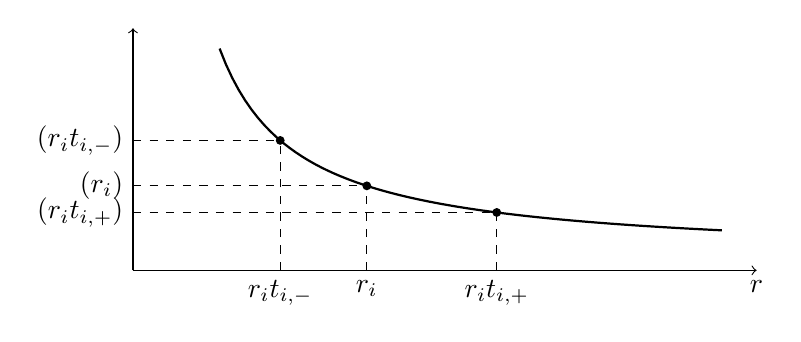
\begin{tikzpicture}[x=1.1cm,y=0.75cm]
\draw[->] (0,0) -- (7.2,0) node[below] {$r$};
\draw[->] (0,0) -- (0,4.1);
\draw[thick,domain=1.0:6.8,samples=80] plot (\x,{3.2/(\x-0.1)+0.2});
\node[right] at (6.8,0.69) {$\tracetwopoint$};
\foreach \xx/\yy/\lab/\vlab in {1.7/2.2/{r_it_{i,-}}/{\tracetwopoint(r_it_{i,-})},2.7/1.4308/{r_i}/{\tracetwopoint(r_i)},4.2/0.9805/{r_it_{i,+}}/{\tracetwopoint(r_it_{i,+})}}{
  \draw[dashed] (\xx,0) node[below] {$\lab$} -- (\xx,\yy);
  \draw[dashed] (0,\yy) node[left] {$\vlab$} -- (\xx,\yy);
  \fill (\xx,\yy) circle (1.6pt);
}
\end{tikzpicture}
\caption{The squeeze. Only $\tracetwopoint$ is monotone (Lemma~\ref{lem:I1.2}). For lattice-rounded separations $t_{i,\pm}\to t_\pm$, $t_-<1<t_+$, the outer values, times $r_i^8\log^2(1/r_i)$, tend to $\traceamplitude t_\pm^{-8}$ along the radii of Lemma~\ref{lem:I-radii}; letting $t_\pm\to1$ gives the limit $\traceamplitude$. Every null sequence has such a subsequence.}\label{fig:I-squeeze}
\end{figure}

\begin{proof}[Proof of Theorem~\ref{prop:TR}]
The phase-table reflection identity E2 of Definition~\ref{def:E1-E3} and the reality of $T$ in Lemma~\ref{lem:G3.2} make $e_{\rm tr}$ real. Lemmas~\ref{lem:G3.1}, \ref{lem:G3.2} and~\ref{lem:H2.4} show that $\Theta$ is real and $O(4)$ invariant and that its continued label is Hermitian and Lorentz scalar. Lemma~\ref{lem:I1.1} gives vacuum centering. For the asymptotic, take any prescribed positive null sequence and the subsequence in~\eqref{eq:I-adjustable}. By Proposition~\ref{prop:I-coefficient}, the phase comparison, and the free normalization in Lemma~\ref{lem:G1.1}, every generic pair $x=(x_0,x_1)$ with $|x|<100$ and $\operatorname{sep}_\infty(x)>1/100$, with $x^{(i)}\in r_i^{-1}a_{n_i}\Z^4$ nearest to $x$, satisfies
\begin{equation*}
r_i^8\log^2(1/r_i)\tracetwopoint(r_i|x_0^{(i)}-x_1^{(i)}|)
\longrightarrow\frac{\traceamplitude}{|x_0-x_1|^8}\,.
\end{equation*}
Translation and $O(4)$ invariance (Lemma~\ref{lem:H1.3}) give $S_2^{\xi_*}(\Theta,\Theta;rx_0,rx_1)=\tracetwopoint(r|x_0-x_1|)$. Here $\slope^{-2}(4d_2)^2=1$, so the amplitude does not depend on~$\slope$.

Take $x_0=0$ and $x_1=(t/2,t/2,t/2,t/2)$, with $1/2<t<2$. This pair is generic and has distance $t$. Monotonicity from Lemma~\ref{lem:I1.2} bounds the lower limit at radius $r_i$ by $\traceamplitude/t^8$ for $t>1$, and the upper limit by that expression for $t<1$ (Figure~\ref{fig:I-squeeze}). Let $t\to1$. The limit along this subsequence is $\traceamplitude$. The subsequence criterion gives the full-radius limit. Here $\traceamplitude=3\dimG/\pi^4>0$ since $\dimG\ge1$; identifying it uses $d_2=-\slope/4\ne0$. Thus $\Theta\ne0$.
\end{proof}

The following high-energy law follows from Theorem~\ref{prop:TR} and Lemma~\ref{lem:I1.2}, as proved below.
\begin{lemma}[High-energy trace limit]\label{lem:I1.3}
For every $\varphi\in C_c(\R^4;\C)\cup\mathcal S$,
\begin{equation*}
\lim_{R_{\rm E}\to\infty}R_{\rm E}^{-8}(\log R_{\rm E})^2\int\varphi(\mathbf p/R_{\rm E})\,d\tracespectrum(\mathbf p)
=\frac{\traceamplitude}{1536\pi}\int_{\forwardcone}\minksquare(\mathbf p)^2\varphi(\mathbf p)\,d^4\mathbf p\,.
\end{equation*}
\end{lemma}
\begin{proof}
The rescaled spectral measures are controlled through their Laplace transforms, which the trace law determines (Definition~\ref{def:D16}, Lemma~\ref{lem:I1.2}). Put $\nu_{R_{\rm E}}=R_{\rm E}^{-8}\log^2R_{\rm E}\,\tracespectrum(R_{\rm E}\,\cdot)$. For every future timelike Laplace covector $u$, with the Euclidean pairing $u\cdot\mathbf p$ of item~\ref{def:W0} of Definition~\ref{def:wightman}, which is the Minkowski pairing of $\mathbf p$ with the future timelike $(-u^1,-u^2,-u^3,u^4)$, Lorentz invariance reduces its transform to the time-axis transform at $s=\sqrt{\minksquare(u)}$. Hence
\begin{equation*}
\int e^{-u\cdot\mathbf p}\,d\nu_{R_{\rm E}}
=R_{\rm E}^{-8}\log^2R_{\rm E}\,\tracetwopoint(s/R_{\rm E})
\longrightarrow \traceamplitude s^{-8}\,.
\end{equation*}
To identify the constant, write $t=\mathbf p^4$ and integrate the spatial radius $q$:
\begin{equation*}
\int_{\forwardcone}e^{-st}\minksquare(\mathbf p)^2\,d^4\mathbf p
=4\pi\int_0^\infty e^{-st}\int_0^t q^2(t^2-q^2)^2\,dq\,dt
=1536\pi s^{-8}\,.
\end{equation*}

The $s=1$ transform bounds compact masses, so diagonal extraction and Riesz representation~\cite[Theorem~2.14]{Rudin1987} give vague subsequential limits. The $u/2$ transform controls the $u$-damped tail, so every limit has the displayed transforms. Holomorphic uniqueness in each coordinate for timelike real part, then Fourier inversion on product Schwartz tests against the finite damped measures~\cite[Theorems~10.18 and~9.11]{Rudin1987}, identify every limit with the cone density in the statement.

For Schwartz tests positivity gives
\begin{equation*}
\nu_{R_{\rm E}}\{\mathbf p^4\le R\}\le e\,R_{\rm E}^{-8}\log^2R_{\rm E}\,\tracetwopoint((R_{\rm E} R)^{-1})\le CR^8
\qquad(R\ge1,\ R_{\rm E}\ge R_{{\rm E},0})\,.
\end{equation*}
Use the trace law at $1/(R_{\rm E}R)$ and $\log R_{\rm E}\le\log(R_{\rm E}R)$. A Schwartz bound of order greater than eight sums the dyadic energy tails uniformly, since $|\mathbf p|\le\sqrt2\mathbf p^4$ on the cone. The $C_c$ limit then gives the Schwartz limit.
\end{proof}

For $\psi_{R_{\rm E}}(x,y)=R_{\rm E}^8\psi(R_{\rm E}x,R_{\rm E}y)$, $\wavetransform\psi_{R_{\rm E}}(\mathbf p)=\wavetransform\psi(\mathbf p/R_{\rm E})$. For $\psi\in\mathcal S_2$, $\wavetransform\psi\in\mathcal S$. Substitution in Lemma~\ref{lem:I1.3} gives the position-space consequence
\begin{equation*}
R_{\rm E}^{-8}\log^2R_{\rm E}\,W_2^{\xi_*}(\Theta,\Theta;\psi_{R_{\rm E}})
\longrightarrow\frac{\traceamplitude}{1536\pi}\int_{\forwardcone}\minksquare(\mathbf p)^2\wavetransform\psi(\mathbf p)\,d^4\mathbf p\,.
\end{equation*}

\subsection{Precise non-free comparisons}\label{sec:partII-I.2}

A finite Wick profile of Definition~\ref{def:D17} is, at small distance, a finite sum of terms $r^a\log^kr$ with $a\in\Z$ and $k\ge0$, plus a bounded remainder; the trace law requires the negative logarithmic power $\log^{-2}(1/r)$. This gives the following exclusion; its proof follows.
\begin{lemma}[Finite Wick obstruction]\label{lem:I2.1}
For every finite Wick profile $W_{\rm Wick}$ and every $\delta>0$, there is $r\in(0,\delta)$ such that
\begin{equation*}
\tracetwopoint(r)\ne W_{\rm Wick}(r)\,.
\end{equation*}
\end{lemma}
\begin{proof}
We expand each profile at small~$r$ and compare with the positive limit of Theorem~\ref{prop:TR}. For one factor, polar coordinates and $\omega_{m_{\rm sh}}=\sqrt{m_{\rm sh}^2+q^2}$ give
\begin{equation*}
K_{m_{\rm sh},k_E,h_{\rm mom}}(r)
=\frac12\left(\int_{S^2}h_{\rm mom}\right)
\int_{m_{\rm sh}}^\infty \omega_{m_{\rm sh}}^{k_E}(\omega_{m_{\rm sh}}^2-m_{\rm sh}^2)^{(j_h+1)/2}e^{-r\omega_{m_{\rm sh}}}\,d\omega_{m_{\rm sh}}\,.
\end{equation*}
For $m_{\rm sh}=0$ this is proportional to $r^{-j_h-k_E-2}$. Otherwise split at $2m_{\rm sh}$; the bounded interval is analytic. On the tail expand $(1-m_{\rm sh}^2/\omega_{m_{\rm sh}}^2)^{(j_h+1)/2}$. Taking enough terms makes the remainder integrable with any prescribed number of energy moments, hence gives a Taylor remainder of the required order. The retained terms are $I_a(r)=\int_{2m_{\rm sh}}^\infty v^ae^{-rv}\,dv$, $a\in\Z$. Integrate explicitly for $a\ge0$; $I_{-1}'=-e^{-2m_{\rm sh}r}/r$ gives the logarithm, and $I_a'=-I_{a+1}$ gives all lower powers. Only nonnegative logarithmic powers occur. For products, choose each remainder order above the other factors' pole orders.

Thus $\operatorname{Re}W_{\rm Wick}=\sum_{a,k}c_{a,k}r^a\log^kr+O(1)$ with finitely many terms. After multiplying by $r^8\log^2(1/r)$, the terms with $a>-8$ vanish. Among the others, the least $a$, then largest $k$, gives a nonzero divergent leading term. A finite limit is therefore zero. Lemma~\ref{lem:I1.2} makes $\tracetwopoint$ real, so equality with $W_{\rm Wick}$ implies equality with its real part. The positive trace limit contradicts equality on $(0,\delta)$, proving also Proposition~\ref{prop:NF}.
\end{proof}

To describe polynomial mass-shell Wick contractions, put $q_m(\mathbf k)=(\mathbf k,\sqrt{m^2+|\mathbf k|^2})$, $m\ge0$. Fix a finite set of elementary field indices, with elements $\mathsf x,\mathsf x'$; words $u,u'$ list its elements. For words of length $k$, $\pi$ ranges over permutations of $\{1,\ldots,k\}$. Comparison data specify finite mass--polynomial lists $\mathcal M_{\rm pair}(\mathsf x,\mathsf x')$, with $P\in\C[\mathbf p^1,\ldots,\mathbf p^4]$, and complex contraction coefficients $c(u,u',\pi)$.
\begin{definition}[Polynomial mass-shell pairings]\label{def:D28}
Set
\begin{equation*}
v_{m,P}(\mathbf k)=\frac{P(q_m(\mathbf k))}{2\omega_m(\mathbf k)},\qquad
L_{m,P}(\varphi)=\int v_{m,P}(\mathbf k)\varphi(q_m(\mathbf k))\,d^3\mathbf k\,.
\end{equation*}
For words $u=(\mathsf x_i)_{i=1}^k$, $u'=(\mathsf x'_i)_{i=1}^k$, define the convolutions of the functionals $L_{m,P}$ by
\begin{equation*}
\mathsf P(u,u';\varphi)=\sum_\pi c(u,u',\pi)
\sum_{(m_i,P_i)\in\prod_i\mathcal M_{\rm pair}(\mathsf x_i,\mathsf x'_{\pi(i)})}
\int\prod_i v_{m_i,P_i}(\mathbf k_i)\,
\varphi\left(\sum_iq_{m_i}(\mathbf k_i)\right)\prod_i d^3\mathbf k_i\,.
\end{equation*}
For unequal lengths put $\mathsf P=0$. A zero denominator at zero momentum gives value zero.
\end{definition}
For finite polynomial fields $Q=\sum_i\alpha_i u_i$, including empty words, the bilinear pairing is $W^{\rm pol}(Q,Q';\varphi)=\sum_{i,j}\alpha_i\alpha'_j\mathsf P(u_i,u'_j;\varphi)$. Empty contractions evaluate $\varphi$ at zero. The shell measure has no $(2\pi)^{-3}$ factor.

The next lemma separates each comparison by one product test; its proof follows.
\begin{lemma}[Polynomial countertest]\label{lem:I2.2}
For every comparison data and every $Q,Q'$, there are $f,h\in\mathcal S$ with compactly supported $\wavetransform(\bar f\otimes h)$ such that
\begin{equation*}
\langle\Phi_\Theta(f)\Omega,\Phi_\Theta(h)\Omega\rangle
\ne W^{\rm pol}(Q,Q';\wavetransform(\bar f\otimes h))\,.
\end{equation*}
\end{lemma}
\begin{proof}
Equality for all product tests would identify the two spectral representations, hence $\tracetwopoint$ with a finite Wick profile, which Lemma~\ref{lem:I2.1} excludes. In detail, equality for all product tests implies equality for every $\varphi\in C_c^\infty$: choose $\widehat h_+=\varphi$ and real $\widehat f_+=1$ on its support. Approximate $e^{-r\mathbf p^4}$ by compact cutoffs. Dominated convergence applies: Lemma~\ref{lem:I1.2} controls $\tracespectrum$; exponential damping controls comparison polynomials at infinity, and $d^3\mathbf k/|\mathbf k|$ is integrable at zero. Expanding the numerators into monomials factors the integrals into the kernels of Definition~\ref{def:D17}, with the empty words giving constants. Hence $\tracetwopoint(r)=W_{\rm Wick}(r)$ for all $r>0$, contrary to Lemma~\ref{lem:I2.1}.
\end{proof}

For the photon comparison use Hilbert tensor products.
\begin{definition}[Ambient and physical Maxwell Fock spaces]\label{def:D29}
For $n\in\N$ colours put
\begin{gather*}
d\sigma(\mathbf k)=\frac{d^3\mathbf k}{2|\mathbf k|},\qquad
\Pi_{ab}(\mathbf k)=\delta_{ab}-\frac{\mathbf k_a\mathbf k_b}{|\mathbf k|^2},\\
\mathcal K_n=L^2(d\sigma;\C^n\otimes\C^3),\qquad
\mathcal F_n=\bigoplus_{k\ge0}\mathcal K_n^{\otimes k},\qquad
\mathcal F_n^{\rm phys}=\bigoplus_{k\ge0}\operatorname{Sym}^k(\Pi\mathcal K_n)\,.
\end{gather*}
The measure has no atom at zero momentum, so the value of $\Pi$ there is immaterial, and $\Pi$ acts pointwise almost everywhere. Thus a physical vector is symmetric and transverse in each slot. Translations multiply sector $k$ by $\exp\{iz\cdot\sum_j(\mathbf k_j,|\mathbf k_j|)\}$. The sector-zero unit is $\Omega_0$.
\end{definition}
\begin{definition}[Coherent comparison vectors]\label{def:D30}
For Schwartz tests $h=(h_{\alpha,a})$, put
\begin{equation*}
v_h(\alpha,a;\mathbf k)=|\mathbf k|\sum_b\Pi_{ab}(\mathbf k)\widehat h_{\alpha,b,+}(\mathbf k,|\mathbf k|),\qquad
\mathcal E(h)=e^{-\|v_h\|^2/2}\bigoplus_{k\ge0}\frac{v_h^{\otimes k}}{\sqrt{k!}}\,.
\end{equation*}
A comparison $U:\mathcal H\to\mathcal F_n$ is a complex linear isometry with image in~$\mathcal F_n^{\rm phys}$, $U\Omega=\Omega_0$, intertwining translations. Set $\psi_U(f)=U\Phi_\Theta(f)\Omega$.
\end{definition}
Real tests have real components. Causal separation means $\minksquare(x-y)<0$ for every pair of points in their closed supports, where $\minksquare(x)=(x^4)^2-\sum_{a=1}^3(x^a)^2$.

Lemma~\ref{lem:I2.2} compares two-point functions only. The Fock test asks more: an embedding of the interacting states into photon Fock space under which the trace field is local relative to the free Maxwell field. Relative locality would impose the equality excluded below. Formally, let $W(h)$ be Weyl operators of the free Maxwell field with $W(h)\Omega_0=\mathcal E(h)$ and $W(h)^*=W(-h)$. If $U\Phi_\Theta(f)U^*$ commuted with $W(h)$ for $h$ causally separated from $f$, then, since $U^*\Omega_0=\Omega$ and $\iota_4\Theta$ is Hermitian,
\begin{align*}
\langle\mathcal E(-h),\psi_U(f)\rangle
&=\langle\Omega_0,W(h)U\Phi_\Theta(f)U^*\Omega_0\rangle\\
&=\langle\Omega_0,U\Phi_\Theta(f)U^*W(h)\Omega_0\rangle
=\langle\psi_U(\bar f),\mathcal E(h)\rangle\,.
\end{align*}
Weyl operators enter only this motivation. The lemma compares the two matrix elements directly, and its proof uses spectral growth without restricting particle amplitudes.
\begin{lemma}[Fock countertest]\label{lem:I2.3}
For every $n\ge0$ and every comparison $U$, for every ball about zero there are Schwartz $f$ compactly supported in that ball and real compactly supported Schwartz $h_{\alpha,a}$, each causally separated from $f$, such that
\begin{equation*}
\langle\mathcal E(-h),\psi_U(f)\rangle
\ne\langle\psi_U(\bar f),\mathcal E(h)\rangle\,.
\end{equation*}
\end{lemma}
\begin{proof}
The proof combines the spectral representation (Lemma~\ref{lem:I1.2}), the high-energy law (Lemma~\ref{lem:I1.3}) and translation covariance (Lemma~\ref{lem:H2.1}) with the dilation behaviour of local photon amplitudes. Fix a ball and suppose equality always holds.

\emph{Sector amplitudes.} Set $p_j=(\mathbf k_j,|\mathbf k_j|)$ and $p_{\rm tot}=\sum_jp_j$. The convolution argument of Lemma~\ref{lem:I1.2} gives sector amplitudes $Y_{k,s}$, with $s$ listing colour and spatial indices:
\begin{equation}\label{eq:I-sector}
\psi_U(f)_{k,s}=\widehat f_+(p_{\rm tot})Y_{k,s},\qquad
\tracespectrum=(p_{\rm tot})_*\sum_{k,s}|Y_{k,s}|^2d\sigma^{\otimes k}\,.
\end{equation}
Box masses are finite. Cauchy--Schwarz and polynomial spectral growth give integrability against sufficiently high inverse polynomials in each momentum.

The common sector unitary $i^k$ preserves the equality, physical vectors and translations. Write $\mathsf Y=i^kY_{k,s}$.

\emph{Locality and doubling.} Expand the coherent equality in a real parameter multiplying $h$, justified by Cauchy--Schwarz and the exponential series. Polarization and complexification give independent complex slot tests. Transversality removes the projector in contractions with physical waves. Shrink nonnegative unit-integral $f$ to zero. Then $|\widehat f_+|\le1$ and $\widehat f_+\to1$; dominated convergence gives, for $g_j$ supported spacelike to zero,
\begin{equation}\label{eq:I-remote}
\int \mathsf Y(\boldsymbol k)\prod_j\big[|\mathbf k_j|\widehat g_{j,-}(p_j)\big]\,d\sigma^{\otimes k}
=\int\overline{\mathsf Y(\boldsymbol k)}\prod_j\big[|\mathbf k_j|\widehat g_{j,+}(p_j)\big]\,d\sigma^{\otimes k}\,.
\end{equation}
Here $\widehat g_-(p)=\widehat g_+(-p)$; the sector factors $i^k$ give exactly these signs.

Fix other slots and use $g(x,t)=a(x)\eta_\epsilon^{(b)}(t)$, with $\eta_\epsilon$ approximating unit mass and $b=0,1$. If $0\notin\operatorname{supp}a$, these are spacelike for small $\epsilon$. Thus both Cauchy data of~\eqref{eq:I-remote} are supported at zero. Weighted integrability bounds their order by $J$, independently of the other tests.

Each datum depends only on the $J$-jet: multiplication by a cutoff in $B(0,\epsilon)$ leaves the distribution unchanged. For a zero-$J$-jet test, Taylor's formula bounds derivatives through order $J$ by $O(\epsilon)$; let $\epsilon\downarrow0$.

The next paragraph proves a uniqueness implication: a combination of sector amplitudes whose two Cauchy data vanish is zero almost everywhere. It is applied below to a polynomial in the doubling operator applied to~$\mathsf Y$, not to~$\mathsf Y$ itself. The massless wave equation separates the frequency branches from these two Cauchy data away from zero momentum. After smearing other slots, each branch is integrable, bounded and holomorphic in its timelike tube, with continuous real boundary. For such a combination with zero Cauchy data, vanishing persists under small translations of the other spacelike tests. Schwarz reflection and holomorphic uniqueness~\cite[Theorems~11.14 and~10.18]{Rudin1987} make the zero set invariant under adding $\R u$ for every future timelike $u$. These vectors span $\R^4$, giving vanishing at every real translation. Successive Fourier inversion~\cite[Theorem~9.11]{Rudin1987} of the smeared integrable amplitudes gives zero almost everywhere. Countably many shrinking bumps remove the other tests: their transforms are eventually nonzero at each momentum.

Let $D_j\mathsf Y(\boldsymbol k)=\mathsf Y(\mathbf k_1,\ldots,2\mathbf k_j,\ldots,\mathbf k_k)$. In the time-order-$b$ Cauchy datum ($b=0,1$), this substitution gives $2^{-3-b}$ times the datum at $a(x)\mapsto8a(2x)$, from $d\sigma(2\mathbf k)=4d\sigma(\mathbf k)$ and $|\mathbf k|^{1+b}$. Spatial jets of order $l$ scale by $2^{3+l}$, giving eigenvalues $2^{l-b}$. Choose a polynomial that annihilates this finite-dimensional dilation action on both Cauchy jets. The uniqueness implication then makes the same polynomial in~$D_j$ annihilate~$\mathsf Y$: for some $J'$,
\begin{equation}\label{eq:I-doubling}
\prod_{a=0}^{J'-1}(D_j-2^{a-1})\mathsf Y=0\qquad\text{in every slot }j\,.
\end{equation}

\emph{Growth.} For $R=2^l$ let $M_{\mathsf Y}(R)=\int_{|\mathbf k_j|\le R}|\mathsf Y|^2d\sigma^{\otimes k}$. By~\eqref{eq:I-sector} and the trace law,
\begin{equation}\label{eq:I-small-mass}
M_{\mathsf Y}(2^l)\le\tracespectrum\{\mathbf p^4\le(k+1)2^l\},\qquad 2^{-8l}M_{\mathsf Y}(2^l)\longrightarrow0\,.
\end{equation}
For the limit, bound the energy mass by $e\,\tracetwopoint(((k+1)2^l)^{-1})$.

Lagrange interpolation in the commuting $D_j$ splits $\mathsf Y$ into joint eigencomponents $D_j\mathsf Y_{\boldsymbol e}=2^{e_j-1}\mathsf Y_{\boldsymbol e}$. Each is a finite combination of doubled copies, so retains~\eqref{eq:I-small-mass}. Moreover $M_{\mathsf Y_{\boldsymbol e}}(2^l)=2^{2l\sum_j e_j}M_{\mathsf Y_{\boldsymbol e}}(1)$, since $d\sigma(2\mathbf k)=4d\sigma(\mathbf k)$.
If $e_j=0$, contraction preserves box mass, contradicting local square integrability and absence of an atom at zero unless the component vanishes. Equation~\eqref{eq:I-small-mass} excludes $\sum_je_j\ge4$. Thus $e_j\ge1$, $\sum_je_j\le3$, and $k\le3$, with box mass $\le CR^6$ for dyadic $R\ge1$. The vacuum sector vanishes by Lemma~\ref{lem:I1.1} and $U\Omega=\Omega_0$.

Summing~\eqref{eq:I-sector} gives $\tracespectrum\{\mathbf p^4\le R\}\le CR^6$ at dyadic $R\ge1$. Multiplication by $R^{-8}\log^2R$ gives zero in the limit, contradicting Lemma~\ref{lem:I1.3} on a nonnegative compact test in $\{0<\mathbf p^4<1,\ \minksquare(\mathbf p)>0\}$.
\end{proof}

An averaged form of this countertest, in which the coherent vectors are moved by maps that preserve physical inner products and fix the image of~$U$, is Lemma~\ref{lem:I2.4} in Section~\ref{sec:correspondence}.
